%% This is the ctufit-thesis example file. It is used to produce theses
%% for submission to Czech Technical University, Faculty of Information Technology.
%%
%% Get the newest version from
%% https://gitlab.fit.cvut.cz/theses-templates/FITthesis-LaTeX
%%
%%
%% Copyright 2021, Eliska Sestakova and Ondrej Guth
%%
%% This work may be distributed and/or modified under the
%% conditions of the LaTeX Project Public Licenese, either version 1.3
%% of this license or (at your option) any later version.
%% The latest version of this license is in
%%  https://www.latex-project.org/lppl.txt
%% and version 1.3 or later is part of all distributions of LaTeX
%% version 2005/12/01 or later.
%%
%% This work has the LPPL maintenance status `maintained'.
%%
%% The current maintainer of this work is Ondrej Guth.
%% Contact ondrej.guth@fit.cvut.cz for bug reports.
%% Alternatively, submit bug reports into the tracker at
%% https://gitlab.fit.cvut.cz/theses-templates/FITthesis-LaTeX/issues
%%
%%

%%%%%%%%%%%%%%%%%%%%%%%%%%%%%%%%%%%%%%%%%
% CLASS OPTIONS
% language: czech/english/slovak
% thesis type: bachelor/master/dissertation
% colour: bw for black&white OR no option for default colour scheme
%%%%%%%%%%%%%%%%%%%%%%%%%%%%%%%%%%%%%%%%%
\documentclass[english,master,unicode,bw]{ctufit-thesis}

%%%%%%%%%%%%%%%%%%%%%%%%%%%%%%%%%%
% FILL IN THIS INFORMATION
%%%%%%%%%%%%%%%%%%%%%%%%%%%%%%%%%%
\ctufittitle{Název příkladné závěrečné práce} % replace with the title of your thesis
\ctufitauthorfull{Bc. Martin Skalický} % replace with your full name (first name(s) and then family name(s) / surname(s)) including academic degrees
\ctufitauthorsurnames{Skalický} % replace with your surname(s) / family name(s)
\ctufitauthorgivennames{Martin} % replace with your first name(s) / given name(s)
\ctufitsupervisor{doc.\,Ing.\,Damien Zlo,\,Ph.D.} % replace with name of your supervisor/advisor (include academic degrees)
\ctufitdepartment{Katedra softwarového inženýrství} % replace with the department of your defence
\ctufityear{2023} % replace with the year of your defence
\ctufitdeclarationplace{Praze} % replace with the place where you sign the declaration
\ctufitdeclarationdate{\today} % replace with the date of signature of the declaration
\ctufitabstractCZE{Fill in abstract of this thesis in Czech language. Class aptent taciti sociosqu ad litora torquent per conubia nostra, per inceptos hymenaeos. Cras pede libero, dapibus nec, pretium sit amet, tempor quis. Sed vel lectus. Donec odio tempus molestie, porttitor ut, iaculis quis, sem. Suspendisse sagittis ultrices augue.}
\ctufitabstractENG{Fill in abstract of this thesis in English language. Class aptent taciti sociosqu ad litora torquent per conubia nostra, per inceptos hymenaeos. Cras pede libero, dapibus nec, pretium sit amet, tempor quis. Sed vel lectus. Donec odio tempus molestie, porttitor ut, iaculis quis, sem. Suspendisse sagittis ultrices augue.}
\ctufitkeywordsCZE{enter, commma, separated, list, of, keywords, in, CZECH}
\ctufitkeywordsENG{enter, commma, separated, list, of, keywords, in, ENGLISH}
%%%%%%%%%%%%%%%%%%%%%%%%%%%%%%%%%%
% END FILL IN
%%%%%%%%%%%%%%%%%%%%%%%%%%%%%%%%%%

%%%%%%%%%%%%%%%%%%%%%%%%%%%%%%%%%%
% CUSTOMIZATION of this template
% Skip this part or alter it if you know what you are doing.
%%%%%%%%%%%%%%%%%%%%%%%%%%%%%%%%%%

\RequirePackage{iftex}[2020/03/06]
\iftutex % XeLaTeX and LuaLaTeX
    \RequirePackage{ellipsis}[2020/05/22] %ellipsis workaround for XeLaTeX
\else
    \RequirePackage[utf8]{inputenc}[2018/08/11] %this file encoding
    \RequirePackage{lmodern}[2009/10/30] % vector flavor of Computer Modern font
\fi

% hyperlinks
\RequirePackage[pdfpagelayout=TwoPageRight,colorlinks=false,allcolors=decoration,pdfborder={0 0 0.1}]{hyperref}[2020-05-15]

% uncomment the following to hide all hyperlinks
% \RequirePackage[pdfpagelayout=TwoPageRight,hidelinks]{hyperref}[2020-05-15]

\RequirePackage{pdfpages}[2020/01/28]

\setcounter{secnumdepth}{4} % numbering sections; 4: subsubsection



%%%%%%%%%%%%%%%%%%%%%%%%%%%%%%%%%%
% CUSTOMIZATION of this template END
%%%%%%%%%%%%%%%%%%%%%%%%%%%%%%%%%%


%%%%%%%%%%%%%%%%%%%%%%
% DEMO CONTENTS SETTINGS
% You may choose to modify this part.
%%%%%%%%%%%%%%%%%%%%%%
\usepackage{dirtree}
\usepackage{lipsum,tikz}
\usepackage{csquotes}
\usepackage[style=iso-numeric]{biblatex}
\addbibresource{text/bib-database.bib}
\usepackage{listings} % typesetting of sources
% \usepackage{minted} % typesetting of sources
\usepackage[inkscapeformat=png]{svg} % SVG support

%theorems, definitions, etc.
\theoremstyle{plain}
\newtheorem{theorem}{Věta}
\newtheorem{lemma}[theorem]{Tvrzení}
\newtheorem{corollary}[theorem]{Důsledek}
\newtheorem{proposition}[theorem]{Návrh}
\newtheorem{definition}[theorem]{Definice}
\theoremstyle{definition}
\newtheorem{example}[theorem]{Příklad}
\theoremstyle{remark}
\newtheorem{note}[theorem]{Poznámka}
\newtheorem*{note*}{Poznámka}
\newtheorem{remark}[theorem]{Pozorování}
\newtheorem*{remark*}{Pozorování}
\numberwithin{theorem}{chapter}
%theorems, definitions, etc. END
%%%%%%%%%%%%%%%%%%%%%%
% DEMO CONTENTS SETTINGS END
%%%%%%%%%%%%%%%%%%%%%%

\begin{document}
\frontmatter\frontmatterinit % do not remove these two commands


\includepdf[pages={1-}]{assignment-include.pdf} % replace that file with your thesis assignment provided by study office

\thispagestyle{empty}\cleardoublepage\maketitle % do not remove these three commands

\imprintpage % do not remove this command

\tableofcontents % do not remove this command
%%%%%%%%%%%%%%%%%%%%%%
% list of other contents: figures, tables, code listings, algorithms, etc.
% add/remove commands accordingly
%%%%%%%%%%%%%%%%%%%%%%
\listoffigures % list of figures
\begingroup
\let\clearpage\relax
\listoftables % list of tables
\lstlistoflistings % list of source code listings generated by the listings package
% \listoflistings % list of source code listings generated by the minted package
\endgroup
%%%%%%%%%%%%%%%%%%%%%%
% list of other contents END
%%%%%%%%%%%%%%%%%%%%%%

%%%%%%%%%%%%%%%%%%%
% ACKNOWLEDGMENT
% FILL IN / MODIFY
% This is a place to thank people for helping you. It is common to thank your supervisor.
%%%%%%%%%%%%%%%%%%%
\begin{acknowledgmentpage}
    Chtěl bych poděkovat především sit amet, consectetuer adipiscing elit. Curabitur sagittis hendrerit ante. Class aptent taciti sociosqu ad litora torquent per conubia nostra, per inceptos hymenaeos. Cras pede libero, dapibus nec, pretium sit amet, tempor quis. Sed vel lectus. Donec odio tempus molestie, porttitor ut, iaculis quis, sem. Suspendisse sagittis ultrices augue.
\end{acknowledgmentpage}
%%%%%%%%%%%%%%%%%%%
% ACKNOWLEDGMENT END
%%%%%%%%%%%%%%%%%%%


%%%%%%%%%%%%%%%%%%%
% DECLARATION
% FILL IN / MODIFY
%%%%%%%%%%%%%%%%%%%
% INSTRUCTIONS
% ENG: choose one of approved texts of the declaration. DO NOT CREATE YOUR OWN. Find the approved texts at https://courses.fit.cvut.cz/SFE/download/index.html#_documents (document Declaration for FT in English)
% CZE/SLO: Vyberte jedno z fakultou schvalenych prohlaseni. NEVKLADEJTE VLASTNI TEXT. Schvalena prohlaseni najdete zde: https://courses.fit.cvut.cz/SZZ/dokumenty/index.html#_dokumenty (prohlášení do ZP)
\begin{declarationpage}
    FILL IN ACCORDING TO THE INSTRUCTIONS. VYPLŇTE V SOULADU S POKYNY. Lorem ipsum dolor sit amet, consectetuer adipiscing elit. Curabitur sagittis hendrerit ante. Class aptent taciti sociosqu ad litora torquent per conubia nostra, per inceptos hymenaeos. Cras pede libero, dapibus nec, pretium sit amet, tempor quis. Sed vel lectus. Donec odio tempus molestie, porttitor ut, iaculis quis, sem. Suspendisse sagittis ultrices augue. Donec ipsum massa, ullamcorper in, auctor et, scelerisque sed, est. In sem justo, commodo ut, suscipit at, pharetra vitae, orci. Pellentesque pretium lectus id turpis.

    Lorem ipsum dolor sit amet, consectetuer adipiscing elit. Curabitur sagittis hendrerit ante. Class aptent taciti sociosqu ad litora torquent per conubia nostra, per inceptos hymenaeos. Cras pede libero, dapibus nec, pretium sit amet, tempor quis. Sed vel lectus. Donec odio tempus molestie, porttitor ut, iaculis quis, sem. Suspendisse sagittis ultrices augue. Donec ipsum massa, ullamcorper in, auctor et, scelerisque sed, est. In sem justo, commodo ut, suscipit at, pharetra vitae, orci. Pellentesque pretium lectus id turpis.
\end{declarationpage}
%%%%%%%%%%%%%%%%%%%
% DECLARATION END
%%%%%%%%%%%%%%%%%%%

\printabstractpage % do not remove this command

%%%%%%%%%%%%%%%%%%%
% SUMMARY
% FILL IN / MODIFY
% OR REMOVE ENTIRELY (upon agreement with your supervisor)
% (appropriate to remove in most theses)
%%%%%%%%%%%%%%%%%%%
\begin{summarypage}
    \section*{Summary section}

    \lipsum[1][1-8]

    \section*{Summary section}

    \lipsum[2][1-6]

    \section*{Summary section}

    \lipsum[3]

    \section*{Summary section}

    \lipsum[2]

    \section*{Summary section}

    \lipsum[1][1-8] Lorem lorem lorem.
\end{summarypage}
%%%%%%%%%%%%%%%%%%%
% SUMMARY END
%%%%%%%%%%%%%%%%%%%

%%%%%%%%%%%%%%%%%%%
% ABBREVIATIONS
% FILL IN / MODIFY
% OR REMOVE ENTIRELY
% List the abbreviations in lexicography order.
%%%%%%%%%%%%%%%%%%%
\chapter{Seznam zkratek}

\begin{tabular}{rl}
    DFA   & Deterministic Finite Automaton                 \\
    FA    & Finite Automaton                               \\
    LPS   & Labelled Prüfer Sequence                       \\
    NFA   & Nondeterministic Finite Automaton              \\
    NPS   & Numbered Prüfer Sequence                       \\
    XML   & Extensible Markup Language                     \\
    XPath & XML Path Language                              \\
    XSLT  & eXtensible Stylesheet Language Transformations \\
    W3C   & World Wide Web Consortium
\end{tabular}
%%%%%%%%%%%%%%%%%%%
% ABBREVIATIONS END
%%%%%%%%%%%%%%%%%%%

\mainmatter\mainmatterinit % do not remove these two commands

%%%%%%%%%%%%%%%%%%%
% THE THESIS
% MODIFY ANYTHING BELOW THIS LINE
%%%%%%%%%%%%%%%%%%%

% Do not forget to include Introduction
%---------------------------------------------------------------
% \chapter{Introduction}
% uncomment the following line to create an unnumbered chapter
% \chapter*{Introduction}\addcontentsline{toc}{chapter}{Introduction}\markboth{Introduction}{Introduction}
%---------------------------------------------------------------

\chapter*{Introduction}
\setcounter{page}{1}
% state the general topic and give some background
% provide a review of the literature related to the topic
% define the terms and scope of the topic
% outline the current situation
% evaluate the current situation (advantages/ disadvantages) and identify the gap
% identify the importance of the proposed research
% state the research problem/ questions
% state the research aims and/or research objectives
% state the hypotheses
% outline the order of information in the thesis
% outline the methodology

Software architecture is the foundation of every application. Like foundation is construction, it has profound effect on the quality of what is build on top of it. As such, it holds a great importance in terms of the successful development and maintenance of the whole system. Architecture serves as a blueprint for a system. It provides an abstraction to manage the system complexity and establish a communication and coordination mechanism among components. Since the dawn of software development, the Monolith architecture has been the industry's favored solution.  However, the increasing complexity of applications has brought to light its limitations in terms of scalability, modularity and maintenance. Since then, there has been a search for a new type of architecture that will overcome these limitations.

Several approaches have been tried, such as Service Oriented Architecture, which seemed promising, but none have matched the popularity of the Monolith. However, more than ten years ago, the Microservices architecture emerged and has spread extensively across the industry, becoming the new standard. Microservices shine at solving the most pressing problem which has risen with constantly increasing number of application consumers, the scalability by allowing to scale horizontally individual parts of the system on demand. The entire application is split into small components with limited responsibility called ``microservice'', which further improves maintenance and makes the system easier to understand.

Unfortunately, Microservices constitute a type of distributed system that introduces significant complexity to the application and complicates deployment. They undoubtedly offer great benefits for sizeable projects with many development teams, yet smaller and medium-sized projects frequently overlook alternative options like Modular architecture. It falls midway between Monolith and Microservices, combining the effortless deployment of Monolith and modularity of Microservices without the complexity of distributed system. The scalability can be achieved later as well by utilizing hybrid approaches.

The objective of this thesis is to elucidate the frequently overlooked disadvantages of Microservices and recommend modern modular alternatives. This is imperative as Microservices can significantly increase project expenses, impede development progress and even result in project failure in the worst-case scenario. The first chapter of the thesis is devoted to a detailed analysis of the Monolith, Modular and Microservices architectures, culminating in a comparative analysis in relation to several factors such as communication, maintenance, deployment and complexity. In the second chapter, an example application is created for each type of architecture and comprehensively analyzed concerning performance and latency. The third chapter presents the authors' personal experience after working over a year on a project utilizing Microservices architecture established four years prior, as well as from personal project that was initially converted to Microservices and then to Modular architecture. The thesis concludes with the creation of a methodology for selecting the appropriate architecture for a new project and how it can be applied and further modified over the course of the application's lifecycle.

% vymezení rozsahu - primárně malé až střední projekty, web-based architecture (not Performance apps)



% The following environment can be used as a mini-introduction for a chapter. Use that any way it pleases you (or comment it out). It can contain, for instance, a summary of the chapter. Or, there can be a quotation.
% \begin{chapterabstract}
%     \lipsum[1]
% \end{chapterabstract}

% \lipsum[1]

%---------------------------------------------------------------
\chapter{Architectures}
\label{chapter:architectures}
In this chapter we will look into classical Monolithic architecture, currently what is considered the most famous called Microservices and what can be found somewhere between: Modulith and Service-Oriented architecture. Apart from defining the architectures, we will compare them among the following lines:
\begin{itemize}
    \item Performance defines how much workload application can handle, how much latency is present during processing and how well application can scale.
    \item Maintainability defines degree to which application is understood, repaired and enhanced from technological perspective.  \cite{SOFTWARE_MAINTAINABILITY}
    \item Sustainability defines how well application performs in long term from business perspective (mainly cost).
    \item Testability defines the extent of how easy or challenging it is to test an application.
    \item Complexity defines how complicated it is to understand the architecture, deployment cycle and implement changes.
\end{itemize}

% Shopify - from Monolith to Modulth https://www.youtube.com/watch?v=ISYKx8sa53g

% System vs application? I want probably refer to app
\section{Monolith}
Probably the most well known architecture praised by some, hated by others is the Monolith.Surprisingly, many people I know do not imagine a properly structured application, but rather `Big ball of mud' \cite{BIG_BALL_OF_MUD} (haphazardly structured, sprawling, sloppy, duct-tape-and-baling-wire, spaghetti-code jungle). Others refer to it as some kind of legacy system that should be eliminated as soon as possible. Of course, there is some truth in all of these statements. Monolithic architecture has been with us since the early days of software development, so there are plenty of legacy systems out there, but we need to understand that they are \textbf{legacy systems}. They were written decades ago, with architectural designs from a time when architectural research was in its early stage. To give some numbers - according to Google Scholar, 20 thousand articles were published about \textit{Software Architecture} until the year 2000 \cite{SCHOLAR_2000} and from 2001 to 2023 it was over 244 thousand \cite{SCHOLAR_2001_2023}. The progress in software architecture has been enormous in the last two decades, and new concepts for monolithic architectures have also been created.

In this section, I'm going to go into detail about what a monolith is, what it isn't, what new approaches are available, and try to clear up some common misconceptions. When I talk about monoliths, I am primarily referring to a unit of deployment\cite{MON_TO_MS_MONOLITH}. \textit{When all functionality in a system has to be deployed together, we consider it a monolith \cite{MON_TO_MS_MONOLITH}.} There are at least three types of monolithic systems that fit this description: the single-process system, the modular monolith, and the distributed monolith \cite{BUILDING_MS_MONOLITH}.


% Starting high level
\subsection{The Single process Monolith}
The most common example of a system where all the code is deployed as a single process, as in Figure~\ref{img:monolith_single_process}. There may be multiple instances of this process running for scalability or availability, but essentially all the code is packed into a single process. Typically, these single-process systems can be simple distributed systems in themselves, as they almost always end up reading data from or writing data to a database. \cite{MON_TO_MS_MONOLITH}

These single-process monoliths probably represent the vast majority of monolithic systems. There is no clear boundary between individual parts and the whole application is highly coupled \cite{EVOLUTIONARY_ARCHITERUES_COUPLING}, meaning that changing one part of the system inevitably affects other parts.

\begin{figure}
    \centering
    \includesvg{images/monolith_single_process.svg}
    \caption{A single process monolith: all code is packaged into a single process. \cite{MON_TO_MS_MONOLITH}\label{img:monolith_single_process}}
\end{figure}


% -------------------------------------------------------
\subsection{The Modular Monolith}
\label{section:modular_monolith}

The modular monolith is a subset of the single-process monolith, where the single process is composed of distinct modules. Although each module can be worked on separately, deployment still requires all modules to be assembled into a single unit, as shown in Figure \ref{img:monolith_single_process_modular}. \cite{BUILDING_MS_MONOLITH}

This is a nice evolutionary step for monolithic systems. Well-defined module boundaries can allow a high degree of parallelism while avoiding the challenges associated with distributed microservice architecture and still having a simple deployment topology \cite{BUILDING_MS_MONOLITH}.

The biggest problem with this architecture is that although the logic is separated into modules, the storage is usually monolithic and represented by a database of relationships. This means that the separation is not effectively applied to the data, but only to the code.


\begin{figure}
    \centering
    \includesvg{images/monolith_single_process_modular.svg}
    \caption{In a modular monolith, the code inside the process is divided into modules. \cite{BUILDING_MS_MONOLITH}\label{img:monolith_single_process_modular}}
\end{figure}


% -------------------------------------------------------
\subsection{The Distributed Monolith}
\begin{quote}
    A distributed system is one in which the failure of a computer you didn’t even know existed can render your own computer unusable. \cite{lamport1987distribution}
    \begin{flushright}
        - Leslie Lamport
    \end{flushright}
\end{quote}

A distributed monolith is a system that consists of multiple services, but for some reason the entire system needs to be deployed together. A distributed monolith may well meet the definition of a service-oriented architecture, but all too often it fails to deliver on the promise of SOA. Distributed monoliths usually have all the disadvantages of a distributed system, and the disadvantages of a single-process monolith, without having enough upsides of either. \cite{MON_TO_MS_MONOLITH}

Distributed monoliths typically arise in an environment where there has been insufficient focus on concepts such as information hiding and cohesion of business functionality, leading instead to highly coupled architectures where changes ripple across service boundaries and seemingly innocent changes that appear local in scope break other parts of the system \cite{MON_TO_MS_MONOLITH}. In general, there is no reason to choose this distributed architecture over microservices, as it has many drawbacks and should be avoided, except when moving from monolith to microservices, where it may become an intermediate step \cite{DIST_MON_WHICH_BUILDING}.

I include this type of monolith for completeness, but since it is discouraged, I will not refer to it unless explicitly stated.

% -------------------------------------------------------
\subsection{Service Oriented Architecture (SOA)}
In the business world, creating solutions to automate the execution of business tasks makes a lot of sense. Throughout the history of IT, such solutions have been built using a common approach of identifying the business task to be automated, defining the business requirements and then building the solution logic \cite{SERVICE_ORIENTED_ARCHITECTURE}. This has been an accepted and proven approach to achieving positive business benefits, but it has had some negative sides:
\begin{itemize}
    \item  Repeatedly building ``disposable applications" is not the perfect approach.
    \item  The creation of new solution logic in a given enterprise typically results in a significant amount of redundant functionality\cite{SERVICE_ORIENTED_ARCHITECTURE}.
    \item Applications built only with the automation of specific business task in mind, are generally not designed to integrate later with other applications well, resulting in a complex integration architecture.
\end{itemize}
All of those negative aspects listed above led to creation of Service-Oriented architecture with the idea of creating reusable services, requiring high-level of interoperability between service and numerous potential service consumers, with standardized contract, loosely coupled and composable, which requires to be standardized with cross-service data exchange.

Service-oriented architecture, or SOA, describes how to use service interfaces to make software components interoperable and reusable. By using an architectural pattern and common interface standards, services can be quickly integrated into new applications. As a result, the application developer is relieved of duties that previously required them to rewrite or replicate existing functionality or figure out how to link or ensure interoperability with it. \cite{IBM_SOA}

In the early days, companies launched major organisation-wide initiatives to convert everything to a service-oriented architecture, which promised many benefits. However, the process was cumbersome and time-consuming, often requiring the company's development team to re-architect all existing systems and design new applications according to new principles. A different way of approaching the problems of SOA was the Enterprise Service Bus (ESB), which can be implemented and deployed in a short time and acts as a central solution for integrations. The ESB approach was quickly adopted and is now used by virtually every company that has an SOA architecture. It allows existing legacy systems to be preserved, simply by exposing services from them via API and creating the integration through the ESB.

Every enterprise contains a service inventory, where all the services are located and from which the target application can be composed, as shown in Figure~\ref{img:soa_architecture}. The directly composable property should have mitigated the traditional perception of integration, but in reality it has just moved into the ESB. Once a significant part of the enterprise solution logic is represented by services in the inventory, the freedom to mix these services into infinite composition configurations to match whatever automation task comes our way \cite{SERVICE_ORIENTED_ARCHITECTURE}.

A classification is used to indicate the reuse potential of the logic and how the service relates to the actual business logic. The common service models are: Task service, Entity service, Utility service and microservice (this is different microservice than we know today, in SOA it was used for small implementation specific service, which was not reusable). \cite{SERVICE_ORIENTED_ARCHITECTURE}

The complexity of implementation to achieve true reusability is huge and has noticeable performance drawbacks, not to mention high maintenance costs. In practice, this architecture has mostly been implemented in large existing companies that already had some legacy systems and combined with the ESB to create huge highly coupled monoliths. Today, everyone is moving away from this architecture, if they have not already done so, towards microservices (section~\ref{section:microservices}), which have proven to be better for the job.

\begin{figure}
    \centering
    \includesvg[width=0.7\textwidth]{images/soa_architecture.svg}
    \caption{Services are delivered into service inventory (right) from which service composition are drawn (bottom). \label{img:soa_architecture}}
\end{figure}

% -------------------------------------------------------

% Going more low level - developer point of view, maybe some example?

\subsection{Characteristics}

\subsubsection{Performance}
\label{section:monolith:performance}
Deploying as a single process gives a huge performance advantage over any kind of distributed system, because network communication is subject to the laws of physics and always adds latency. Inter-process communication, on the other hand, has the lowest possible latency, making the monolith theoretically the fastest architecture out there. This rule applies until the need to scale the application arises and vertical scaling is no longer an option. Since the whole system is deployed as a single unit, horizontal scaling means running multiple instances of the whole monolith, which in most cases is not very efficient, because the system is usually not evenly loaded, but some parts of the system are doing most of the work, and we still have those other parts taking up resources when we don't actually need them.


% latency
% throughput
% scalability
% 

\subsubsection{Maintainability}
Maintenance is closely related to complexity. Usually, the more complex the application, the harder it is to maintain, and with monolithic high coupling it is very bad at it. A single change can have the power to affect the entire application, and maintaining legacy monoliths has become a nightmare for many developers, as even the smallest change requires extensive knowledge of the whole system. Although there are some positive sides, debugging and logging is much easier than with any kind of distributed system, so finding the problem is usually the easy step compared to creating the actual fix.

% Easy debugging | logging

\subsubsection{Sustainability}
% Not sure what should be here
The maintenance costs of monolith are huge, as are the operational costs due to its inability to scale properly, so we have to have an oversized infrastructure, but also developers with extensive knowledge of the system and a well-defined testing process. Introducing any kind of architectural change is almost impossible and integrations have also proven to be complicated/problematic.

\subsubsection{Testability}
Since there are no boundaries in the classic monolith, it is almost impossible to test only certain parts of the system in isolation, because the whole system has to be present for it to work. So writing end-to-end tests is usually the answer, but it is much harder to write and even execute them, because they take much more time than just testing isolated parts.

With a modular monolith, testing is much easier because you can test only specific modules. The tests are smaller, which results in higher speed, and are easier to write because the developer can focus only on the specific part of the system.

\subsubsection{Complexity}
High coupling makes it very hard to do any modification, because it requires vast knowledge of the whole system and as the developer team grows they start to get into each other way, wanting to change the same piece of code. It also creates confusion about who owns the code and who makes the decisions \cite{MON_TO_MS_MONOLITH}.

The architecture itself (single process or distributed monolith) imposes no restrictions on how the application should be structured and gives the developer maximum freedom. In my experience, this has proved fatal in many projects as it is a heavy burden and if not properly designed at the outset and kept under control throughout the development cycle, it can very easily lead to a `big ball of mud' \cite{BIG_BALL_OF_MUD}.

% TODO: Take into account database coupling of records and how Modulth does it
High coupling is one of the reasons why the Modular Monolith was created. It retains all the positive characteristics of the single-process monolith, while reducing the coupling by defining boundaries within the monolith. It is then up to the developers to properly define and enforce these boundaries - this step is very important because less experienced developers often tend to simplify their work at the expense of the architecture.

Deployment is very simple compared to any kind of distributed system, as there is only one unit. The downside is the size of the unit, not even because of space (we have a pretty fast network and cheap disk space), but rather higher resource usage and much slower startup compared to a microservice.

% release complexity
On the other hand, when there are multiple teams working on a monolithic system, release planning requires close cooperation between all development teams to ensure that everything that goes into the build is production ready. This tends to lead to slow deployment cycles, where releases are deployed every few months, which does not cope well with today's requirements to deploy much more frequently (e.g. Agile methodology \cite{AGILE_MANIFESTO}).

% Dev tools stack
\section{Modulith}
\label{section:modulith}
`Microservice architectures are all the rage these days, but what's really important for long-term maintainability is modularity. It isn't necessary to use a network boundary to create such modules.' \cite{HOW_TO_BUILD_MODULAR_MONOLITH_CONFERENCE_INTRO}

The word \textit{Modulith} is combination of words `Modular' and `Monolith'. In previous section was discussed Monolith architectures and one of them was \textit{Modular monolith} \ref{section:modular_monolith}, which basically enforces separation of logic into modules. Modulith is taking this modular approach even further by enforcing separation not just on logic, but on database/storage as well (see Figure~\ref{img:modulith_architecture}). This way the modules are truly independent on each other, and they are in full control of its data, since now modules has to communicate with others via defined interfaces (this can be done for example directly via inter-process communication or messaging). Isolated, independent modules with interface through which they communicate formulate Modulith.

Modules being fully encapsulates give ability to even run different modules on different nodes/servers and communicate with others over the network, I call this \textbf{Hybrid Modulith}, and this is basically what Microservices are in its nature are. It is an enormous evolution compared to classical Monolith in terms of scaling, since this architecture offers ability to scale just parts of the systems (modules) instead of the whole application. Slow transition to Microservices (discussed in following Section \ref{section:microservices}) is natural step, once the need for scaling arise - just by moving required module into separate service we get a hybrid of microservices and modulith. So the whole application can be build using Modulith architecture, keeping all advantages of Microservices and in the same time removing the biggest disadvantage `distributed system' with the ability to incrementally move to distributed system once it is absolutely necessary.

Modulith is a better structured Monolith with ability to scale. It still has the nature of Monolith, so it is deployed as one unit, which gives confidence of matching interfaces across modules, which is something that Microservices architecture is missing, easier debugging as it is not a distributed system and modularity of Microservice architecture for long-term maintainability. To improve deployment time for larger projects, we can deploy modules independently as modern languages generally support dynamic module loading/replacement at runtime, but this adds complexity as we need to ensure that all deployed modules are compatible and perform the update atomically. 

\begin{figure}
    \centering
    \includesvg{images/modulith_architecture.svg}
    \caption{Mondulith architecture. Modules encapsulate logic and its own data. \label{img:modulith_architecture}}
\end{figure}

\subsection{Characteristics}
\subsubsection{Performance}
Running as a single process, gives this architecture near same properties concerning performance as for Monolith \ref{section:monolith:performance} with a little drawback due to its added abstraction and isolation of data storage across modules, but the modularity being huge improvement in long-term maintainability. The Modulith architecture does not scale itself, but rather presume incremental transforming into microservices when the need arises. The right question is how much do we really need our architecture to scale. When starting a project, we can have some expectation on system load, but with how dynamically today project change from nearly from day to day, it usually starts as products A and finishes as product Z, so our presumptions on start will have to be adjusted as well. With that being sad, it is nearly impossible to guess what needs to be scaled beforehand, and rather have architecture, which allows us build fast with minimal overhead and with ability to scale once we actually need it. Also, if we look on modern hardware, we can find affordable up to 128 cores servers, which can easily run our wildest applications even without getting into distributed systems. Programming languages were adapted over the years as well: NodeJS with even loop can handle easily thousands of connections in single thread, Java recently got virtual threads (virtual threads), Golang has goroutines and Rust has asynchronous programming. All of those tools allows writing effective code when dealing with IO taks, which is what most of today applications are mostly made of.

Once we have to scale this architecture, some modules are moved into separated service, heading towards microservices and the negative aspects of distributed system will start appear - mainly the network unreliability and latency, more discussed in Microservice section \ref{section:microservices:performance}.


\subsubsection{Maintainability}
This is where the Monolith has been proved to be very problematic and the Microservice shines. Enforcing modularity on architecture level turned out to be essential in long-term maintenance. In my experience all projects usually begin as beautiful things and over time got messy. In my own opinion this is primarily caused by laziness of us developers. If there is some shortcut we can use, we will and say to ourselves: `I will fix it later', which off course never happens. I am not saying this happens all the time, but there are times, when deadlines start breathing on our neck and forcing us to do things faster. So, when we remove some of those shortcuts as were in Monolith, which allowed to do anywhere anything and force modularity on architecture level as in Modulith, developers has no other choice then to do it properly, since there will be no other way. It does mean that some features will take few minutes or hours more, but this will be well invested time compared to searching for mysterious bugs in Monolith where much, much more time is spent.

\subsubsection{Sustainability}
Modularity provides great flexibility and allows for faster iterations to better adapt to changing business and
requirements and architectural changes.

\subsubsection{Testability}
Testing is very similar to microservices, as the entire application is broken down into modules that can be tested independently. The big advantage even over microservices is the single-process nature, which allows testing using conventional tools and frameworks designed for monoliths.

\subsubsection{Complexity}
In terms of complexity the Modulith architecture sits somewhere between Monolith and Microservice. In its nature it is not a distributed system as Microservices, so there are no network issues and deployment process is as simple as for Monolith. Until we start running modules in separated service, we get partially distributed system, and the complexity arises. The advantages of Modulith is the incremental migration to distributed system and ability to decide whether it is actually needed, because with Microservices we have distributed system from the start even if we want/need it or not. The same applies to the implementation of transactions, until we start moving towards a distributed system the same transaction patterns can be implemented as were for Monolith. Distributed transactions will be discussed later in Microservice section \ref{section:microservices:complexity}.
\section{Microservices}
\label{section:microservices}
Many people consider this architecture as solution for every problem. What architecture for new project? Microservices. Is your application slow? Convert it to Microservices. Experiencing slow development? Microservices are the solution. Fair enough, it really does change the game and there are definitely projects where it is the best possible solution. Although in my experience, people tend to use this architecture carelessly as the only correct solution, ignoring its disadvantages, and there are definitely projects where for example monolith would be more suited for task and save a lot of many and time. So what exactly is it?

\begin{quote}
    Microservices are independently releasable services that are modeled around a business domain. A service encapsulates functionality and makes it accessible to other services via networks—you construct a more complex system from these building blocks. One microservice might represent inventory, another order management, and yet another shipping, but together they might constitute an entire ecommerce system. Microservices are an architecture choice that is focused on giving you many options for solving the problems you might face. \cite{BUILDING_MS_WHAT_ARE}

    They are a type of service-oriented architecture, albeit one that is opinionated about how service boundaries should be drawn, and one in which independent deployability is key. They are technology agnostic, which is one of the advantages they offer. \cite{BUILDING_MS_WHAT_ARE}
\end{quote}


From a technology viewpoint, microservices expose the business capabilities that they encapsulate via one or more network endpoints \cite{MON_TO_MS_MICROSERVICE} (for example, a queue or a REST API \cite{BUILDING_MS_WHAT_ARE}, as shown in Figure~\ref{img:microservices_basic}). Microservices communicate with each other via these networks — making them a form of distributed system. They also encapsulate data storage and retrieval, exposing data, via well-defined interfaces. So databases are hidden inside the service boundary. \cite{MON_TO_MS_MICROSERVICE}

Compared to the discussed Modulith in section \ref{section:modulith}, Microservices are taking the whole modular concept one step further. Instead of primarily building the application around modules with possibility to extract module into separate service to scale it, they are building the whole application from the ground around services with network boundaries fully embracing scalability. This is where I see the problem with building new applications with Microservices architecture from the start when there is no idea about system load, performance issues or just about anything. I would compare it to `Premature optimization' in programming - why spend a lot of time building super scalable system, when we do not even know yet if we will ever need it?

% how to find correct size of microservice
What is the correct size of single Microservice? The \textit{micro} part of the word is misleading. The Microservices were created primarily for needs of big companies and original idea behind it was to have a dedicated team of developers behind nearly Microservices. And this is something, which is not possible in most of the companies with just couple of developers. The practice I have seen in reality is, that just couple of developers are running dozens of microservices or even in one project I was single developer managing over 20 microservices (experience described in Chapter \ref{chapter:personal_experience}). The `micro' just means completely different thing for big companies like Netflix or Amazon and for small/medium projects.

Building Microservice architecture requires a lot of planning to properly set boundaries to individual services and keep an eye on it. It is much harder to do bigger refactoring compared to Monolithic architecture even though it should be easier due to the service isolation. Unfortunately in practice due to business requirements it is impossible to create something completed independent. Example: Lets image we have microservice with some HTTP API, which we need to split. Other service are communicating with it through the API. We need to hold the compatibility for API for a long time, since we most likely do not know exactly which services are using which API and if it is safe to remove anything. So, we split the service, the old service will have the full original API, the new service just the part of the API, which it can handle. For the old service additional backward compatibility logic needs to be implemented for those parts of API, which were moved to second service. And this compatibility needs to be maintained for unspecified period of time - this depend if we have any strategy how to safely remove anything and make sure it does not break other parts of system. On other hand in Modulith we would just split the one module into two, and we very easy find all places which uses the old functionality and update it accordingly - how to find it? IDE (basic feature `find usage'), compiler, static code analyses. The compiler makes sure automatically all interfaces and implementations are compatible, and it does for free out of box. Just something, which is not easily possible in Microservices world.


\begin{figure}
    \centering
    \includesvg[width=0.7\textwidth]{images/Microservices_basic.svg}
    \caption{A microservice exposing its functionality over a REST API and a topic. \cite{BUILDING_MS_WHAT_ARE}\label{img:microservices_basic}}
\end{figure}



\subsection{Brief history}
Dr. Peter Rodgers during a presentation in 2005 used the term `Micro-web-Services' on topic of cloud computing. Redgers promoted software components supporting micro-web-services. The first usage of the term "microservices" is to believed to be first heard in May, 2011, in a workshop for software architects, where they use it to describe an architectural style several of them had recently explored. Later on in 2012, the term was formally adopted. They had been experimenting with building continuously deployed systems, while incorporating the DevOps philosophy. From there this form of architecture quickly gained popularity. \cite{BRIEF_HISTORY_OF_MS}

% TODO add sources
Netlix is a company considered as a pioneer in the field together with Amazon, which was more focusing on Cloud computing. Also, other large companies joined the ride like Uber, Etsy and many more. This architecture was the answer companies were looking for, due to its ability to offer agility, scalability and ability to adapt to changing business requirements. \cite{MS_COMPANIES}



\subsection{Performance}
Microservices being distributed system, it necessarily adds higher latency compared to Monolithic systems, but it brings many advantages which can easily balance this negative side. The biggest being the scalability. Microservices are very small unis, which can usually start up in couple of seconds, so it can be scaled based on current workload fully leveraging cloud computing and pricing per usage rather having oversized infrastructure. On other hand scaling does not work out of the box and it requires system to support it. Also, it is not possible to scale up infinitly and some bottleneck will stand out, usually being database.


\subsection{Maintainability}
% Distributed tracing
Distributed system are much harder to maintain due to added complexity. Even thing like investigating some issue requires collecting logs from multiple servers, aggregating them together and having tool to effectively search through it. Or even better way is to use Distributed tracing, which can generate vast amount of data even on simple systems.

\subsection{Sustainability}

\subsection{Testability}
In theory testing should be breeze, but in really not so much, because services are usually part of a larger business-logic dependent on other services to complete the logic. Practices for service-testing (e.g. mocks, API-contract testing) are known, but they are very complex and costly to implement. In comparisement for monoliths we have many proved testing strategies including end-to-end with many great frameworks/libraries available. \cite{MC_TESTABILITY}

Service can often become inaccessible, due to issue on many layers of network or security operated by an orchestrating software. These kinds of problems are hard to simulate in-order to prevent faults from reaching production.

\subsection{Complexity}
% orchestrator + deployment
Breaking whole system into isolated `micro' pieces (services) makes it easier for developers to implement new features and work independently, but it definitely makes the whole system more complicated, because of added network communication and more complicated deployment. Network communication is required for inter-service communication and also for outside world, and there is a lot we can choose from. Starting from classical patterns like request-response or more data driven approaches like observer or publish-subscribe.
% TODO dive more deep into communication 

Managing deployment of microservices is a big task and over the years lot of automation tools were created. Today standard way on how to deploy applications with rise of Docker became containers, due to its self-containement, isolation and ability to run absolutely anywhere \cite{7093032}. Container Orchestration make deployment and maintenance much easier thanks to automatization - examples: Kubernetes\cite{KUBERNETES}, Nomad\cite{NOMAD}. It takes care of whole lifecycle of the application and even auto-scaling. Unfortunately, managing those tools is a big challenge on its own, but thankfully nowadays we can get fully managed orchestrators `as a Service', so we can fully focus on building our system and not on infrastructure.

% TODO more deep into example technology stack - maybe later in comparison chapter

% Distributed transactions
Distributed transactions have the same processing requirements as regular database transactions, but they must be managed across multiple resources, making them more challenging to implement. When ACID transactions are required, the 2PC \cite{2PC_PATTERN} (two-phase commit) architecture with central transaction coordinator is a one solution. On the other, hand if eventual consistency is enough, there is SAGA pattern \cite{SAGA_PATTERN}, which works sequentially.

% language and technology agnostic
Language and technology-agnostic is another advantage presented around Microservices. A personally perceive it as negative for small teams, where few developers manages dozens of Microservices and they would have to constantly switch context. But it is great trait for large teams, where ideally one team has just one or couple of microservices. It gives a lot of freedom and developers like to play with every new shining piece of software/technology, which can result (if unchecked) in technology jungle to which no one understands and is unable to maintain. The same applies for languages. Although I am strong advocate for always using language for the right task, it must be well argued and everyone on the team should be familiar with it, because in small teams there is usually shared code ownership.


\section{Summary matrix}
Following table~\ref{table:architecture_compare} contains summary of previous sections discussing multiple architectures.

% TODO - add tooling complexity

\begin{sidewaysfigure}
    \begin{tabular}{ |p{2.7cm}|p{3cm}|p{3cm}|p{4cm}|p{3cm}| }
        \hline
        \textbf{Aspect}       & \textbf{Monolithic}                            & \textbf{Modulith}                                 & \textbf{Hybrid Modulith}                                                            & \textbf{Microservices}                                                                        \\
        \hline
        Structure             & Single, highly coupled   application.          & Single, loosely coupled application               & Multiple loosely coupled Moduliths.                                                 & Many small, independent services.                                                             \\
        \hline
        Communication         & Direct function calls.                         & Direct function API calls.                        & Network communication.                                                              & Lof of network communication.                                                                 \\
        \hline
        Scalability           & Add instance of whole application.             & Add instance of whole application.                & Add instance of individual Modulith.                                                & Add instance of individual microservice.                                                      \\
        \hline
        Architecture overhead & Minimal                                        & Minimal                                           & Moderate                                                                            & Higher                                                                                        \\
        \hline
        Maintainability       & Modification can affect the entire application & Modification in modules has isolated effects. *   & Modifications in module have isolated effect. *                                     & Modifications in microservice have isolated effect. *                                         \\
        \hline
        Deployment            & Single unit.                                   & Single unit or independent deployment of modules. & Independent deployment of Moduliths or individual modules.                          & Independent deployment of microservices.                                                      \\
        \hline
        Collaboration         & Everyone works on one codebase.                & Everyone works on one codebase.                   & Teams collaborate on individual Moduliths.                                          & Teams collaborate on individual microservices.                                                \\
        \hline
        Complexity            & Higher due to highly coupled  components       & Lower complexity with highly decoupled modules.   & Moderate complexity with decoupled modules (lightly fragmented distributed system). & Higher complexity with highly decoupled microservices (highly fragmented distributed system). \\
        \hline
    \end{tabular}
    \caption{Overview of architectures. *Modifications to API always affects the whole application.\label{table:architecture_compare}}
\end{sidewaysfigure}


%---------------------------------------------------------------
\chapter{Financial well-being project}
\label{chapter:personal_experience}
In this chapter we'll take a closer look at one of the projects I've worked on that was built from the ground up using a microservices architecture. I will share my experience from the position of a backend developer on what it means to work on microservices architecture alone and in a team. What are the downsides and upsides for developers during the whole application cycle (planning, implementing, deployment, maintenance).

\section{Personal experience with Microservices}
At the time of writing, I have been working for the company for over a year on their financial wellbeing platform. The purpose of the platform is to help users connect with coaches and give them tools to educate themselves, get their finances under control and plan for the future.

This project has been in development for over 4 years with only a handful of developers. The backend is written using microservices architecture in Rust and there are 2 frontend applications: native iOS and web. There are also two additional web frontends for administration. Admin portal is used by financial advisors to communicate with users and also by support/admin users. The latter is the customer portal, available to our customers (employers) to see their employees' interactions with our platform.

\subsection{User journey}
Over the years the platform has gained a lot of features, so I will just highlight the main ones to give you an idea of what the platform does. I will describe the processes using user journeys:

\begin{example}[Sign Up]
    Joe, an employee of company Z, receives an email about gaining access to the platform, which his employer has purchased as a benefit. Joe opens a web browser and goes to the registration page. He enters his email and password and goes through the onboarding process (a few basic questions about his financial experience and goals). Once registration is complete, he lands on the home page.
\end{example}

\begin{example}[Advisor]
    Immediately after signing up, Joe is presented with the name of his personal financial advisor. He can send him a message via chat, or better still, schedule a phone call so they can meet face-to-face, get to know Joe's expectations, review his finances and set some goals.
\end{example}

\begin{example}[Analyse]
    Meanwhile, as Joe waits for his first meeting with his adviser, the platform offers to connect his bank accounts so it can give him some insight into his spending. In the UK, there is an open banking standard that allows him to give the application access to his accounts and transactions in just 3 steps. Once connected, Joe is presented with graphs showing how much he spends each month in each category. He can also set goals (e.g. wedding or buying a house), link them to accounts and it will automatically track any progress (savings).
\end{example}

\begin{example}[Education]
    On the Learning page, Joe can read thousands of financial articles written by our financial advisors or watch recordings of past webinars. He can also view and register for upcoming webinars.
\end{example}

% \subsection{Vocabulary}
% Before moving into technical side of the thing, we need to first define few terms, which will be used throughout this chapter:
% \begin{description}
%     \item[Insight]
% \end{description}


\subsection{Infrastructure}
The infrastructure is based on HashiCorp products (HashiStack). The cloud provider is used for VM provisioning and networking, but they manage the rest themselves via custom Terraform scripts (IaaS). What are the key components:
\begin{itemize}
    \item \it{Nomad} is a simple and flexible scheduler and orchestrator for deploying and managing containers. \cite{NOMAD}
    \item \it{Consul} is a service networking solution that automates network configuration, service discovery and secure connectivity. \cite{CONSUL}
    \item \it{Vault} secures, stores and tightly controls access to tokens, passwords, certificates, API keys and other secrets critical to modern computing. \cite{VAULT}
\end{itemize}

I don't know what the reason was for going with the HashiCorp stack, but looking at the experience with it after a year, I'm amazed at how well the components integrate, and the setup/management of the whole cluster was a breeze compared to Kubernetes (K8s). There are now many managed K8s clusters available, but not a single managed Nomad cluster provider that I could find (there was an unmanaged.io project, but it seems to be down). I think the reason for this is simple - Nomad is just easy to run and manage. I'm not condemning K8s, I'm sure the complexity is there for a reason, but just for this project Nomad was more than enough and much easier to work with. During the year we had 2 incidents in production. The first was caused by a weird cluster state, which was resolved by rebooting, and the second was caused by our cloud provider having network issues. As we had no one dedicated to infrastructure and everything was managed by the BE developers, we just needed something that was easy to use and would work. Nomad did exactly that without adding any complexity that we did not need and that K8s would most likely add.

Compared to this relatively simple microservices infrastructure, it still consists of a lot of components that new developers need some time to get used to. A few examples:
\begin{enumerate}
    \item The API gateway was created using a proxy called \textit{fabio}, which has it's own way of defining path mapping.
    \item Nomad has it's own job definition language called HCL.
    \item The inter-service communication needs to be protected because it is over the network. So additional secrets handling and service discovery had to be done before each inter-service call.
    \item Changing deployment features requires knowledge of devops and editing not-so-simple pipelines.
\end{enumerate}
None of the above examples of obstacles exist when working with monoliths.



\subsection{Microservices}
The whole platform consists of 26 microservices, 4 of which are backend for frontend. Each microservice exposes its API via HTTP protocol for inter-service communication as well as to the outside world and API Gateway is created via reverse proxy called \textit{fabio}. For background tasks, a messaging system with queues is used, specifically Amazon's SNS for sending messages and SQS for receiving them.

Git is used for versioning with one repository per microservice. I see some advantages in having separate repositories compared to monorepo. Firstly, pull requests are better organised and compact - changes to a microservice should be isolated, and having Monorepo allows code in multiple microservices to be touched, and it would be up to the code reviewer to notice. It also forces developers to think of changes as more isolated, since they can only change a single microservice in a single repository - they have to switch to another to make the next changes. The same flow could be enforced by git hooks, for example, but this way it requires no configuration. On the other hand, it is a bit harder for newcomers to simply download all repositories, as 26 is quite a lot and requires some structure to be added to local repositories for easier navigation.

Finding the right size of microservices is a difficult task. In this project, the domain driver approach was used to find 'small enough pieces' (this was approximated) and map them into microservices. Some have well defined boundaries, some have a grey area, few are overgrown and should have been split because maintenance has become much harder with increasing complexity. A few examples:

\begin{itemize}
    % TODO add more examples
    \item \it{Financial Account} holds information about bank accounts for users. Either manually created accounts or those that are connected.
    \item \it{Transaction} stores financial transactions.
    \item \it{Categorisation} contains pure logic that categorises transactions into different categories.
    \item \it{Orchestrator} is used for scheduled tasks that trigger complex flows involving multiple microservices, such as updating cached accounts and Open Banking transactions, and starts the post-processing.
    \item \it{Advisor} was designed to hold the logic and data around advisors and their relationship with users. Later, chat functionality was added, and as it started with just basic messaging between advisors and users, the unfortunate decision was made to include everything around messaging here as well. Over time, this functionality has been extended and this microservice has become the most bloated of all.
\end{itemize}

From the examples above, it is clear that microservices have varying scopes/boundaries. Even if we have the best possible design at the start, over time, features will change and this will inevitably lead to an uneven distribution of boundaries. This does not mean that there is a problem with the design, as our system might just be adapting to our changing business needs, shifting goals, and our design needs to adapt as well. There are usually two outcomes. The first is a proper adaptation of the design, once we realise that the change is needed, and with it a possible refactoring/split/merge of microservices. The second option is what happened to the Advisor service. Over time, it took on more and more functionality, even outside its scope, and when someone later realised the mistake, the amount of work required to make the necessary changes was simply too much to invest at the time.
% how is this possible? Microservice from definition is independent and isolated, so it should be easy just to split into two. Well, even though definitions sound great, the complexity always depends on the actuall implementations. 
% - contracts (swaggers)
% - compatibility
% ability to remove something from contract
% tracking dependency

\subsubsection{Complexity}
% TODO it gets complicated - need to expose lot of APIs (+ maintanance), hard to solve security 
The idea of having lots of micro independent services is great from a scaling and rapid deployment perspective, but as with everything, there are negatives. Each service defines its own interface, in this case as a Swagger definition, and is kept in sync with the code manually, which inevitably leads to problems. There are some automated solutions that either generate the OpenApi definition from the code or vice versa. Unfortunately, it has some limitations, not every language has support for it, and I have not seen any project that actually uses it and relies on it completely. These outdated contracts have led to confusion for front-end developers, an inability to rely on it, and in practice, every time a front-end developer needed detailed behaviour about an endpoint, he had to contact a back-end developer who would investigate the behaviour directly from the code. Today, gRPC technology would probably be better for inter-service communication, as it has support for every major language and can automatically generate either server or client implementations from schema.

Defined contracts, whether via OpenApi or any other technology, ideally need to be maintained indefinitely, which is of course not possible. Even with the best design in mind, requirements will change, features will become obsolete, and maintaining each obsolete/old/unused feature will take a lot of time. In monolithic/modular statically typed systems, when someone changes the interface/contract, the compiler gives instant feedback as to whether these changes can be made, or whether there are conflicts, and where exactly. In the world of microservices, this is a much more complex issue. Taken to the extreme, each service implements its own client to communicate with all dependent microservices. When this happens, as it did in this project, how can you tell if even a specific change as small as removing a single field on the contract will affect other microservices, if any? Perhaps using an advanced static code analysis tool for this specific purpose would give an idea, but I doubt it would be reliable. Another option I took after seeing this, also code duplication with this approach, was to publish the client implementation with each contract change. That way, other microservices could simply add the client library as a dependency instead of implementing their own. Tracing dependencies between services was now as simple as checking dependencies and looking for client libraries. Now at least the incompatible changes to contracts are at least somewhat possible, as a new version of the client library can be released and each microservice can be rebuilt (e.g. as part of CI) with the updated client library to see its impact.

Leveraging our existing code convention across services, I was able to generate a dependency graph for the whole system via static analysis, see graph \ref{img:microservices-current-commented} (something that was not available and no one paid attention to). This is a real example of what can happen to a microservices architecture after 3 years of development, and this graph does not include communication via async messages. It is not easy to say whether the state looks bad or not, but I would lean towards bad after seeing the graph. If this were the module dependency graph of Modulith, it would take some time to make changes, but once done and the compiler was happy, it would be done. But if someone wants to do these big kind of changes like change contracts (internal just between services) in microservices it is much more work having to change contract, client implementation, propagate the change to every service where it is used. Just to see where it is used is a task on its own compared to a single process system where every IDE is fully capable of showing you in a matter of seconds every single usage in the codebase. And the worst part is the inability to properly check if all the contracts for each service are fully compatible and will work, or if there is simply a typo somewhere, or if during refactoring a service was simply left out, which actually happened from time to time. Even though we had the code coverage, the tests were still expecting the older version of the contract, so the problem would show up once it was running in the real environment. At best we would catch it in development, at worst it would show up in production after release.

\begin{figure}
    \centering
    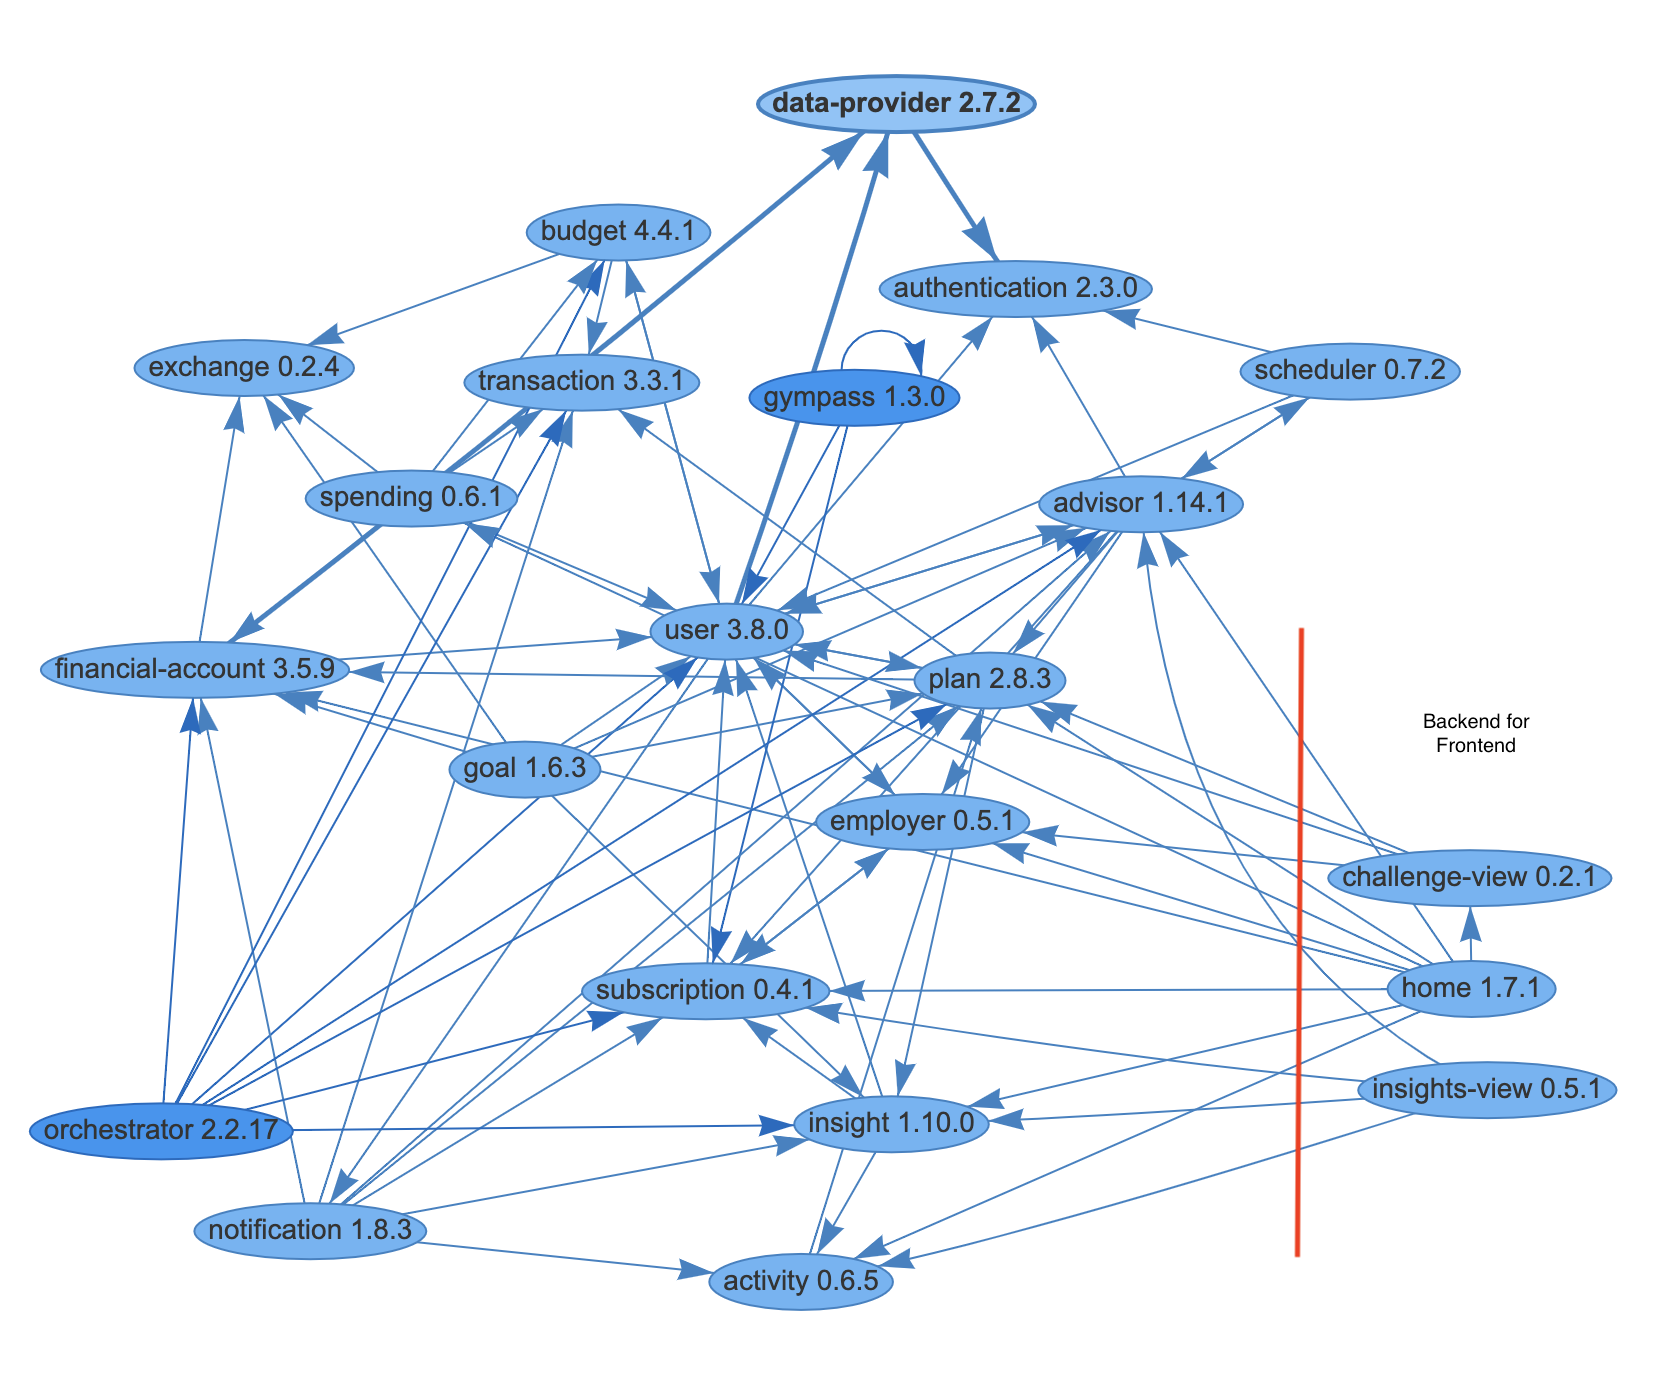
\includegraphics[width=\textwidth]{images/microservices-current-commented.png}
    \caption{Inter microservice dependency graph of backend after roughly 3 years of development. \label{img:microservices-current-commented}}
\end{figure}

% TODO popsat deployment complexity
% Popsat stroze flow, víc to rezipíšu obecně v Analyse chapter
In terms of performance, there were only two services that had noticeable CPU usage and those were processing thousands of financial transactions every time the user opened the analysis page, the rest was mainly waiting for the database to read or write data. Despite this, we had very linear traffic and each service was only running in two instances with no autoscaling and only a few hundred MHz of CPU allocated to it, so it was almost like Monolith with two instances, with the exception that even internal requests were load balanced and not just external as with Monolith. So in this case, it would easily run as a monolithic system without any problems, with plenty of room to grow vertically: with 26 microservices, each would have 500\.HMz of CPU and 100\.MB of memory allocated. The total resource requirement for a single monolithic instance would be 5~CPU cores (2\.GHz per core) and 1\.GB of memory.

% Working on bigger feature it meant touching multiple services. Later the deployment required to check all not-deployed work and figuring out what has been tested and can be deployed to production. This flow is most likely the same for all projects, just for Microservices it is easier compared to Monolithic since the change are usually much smaller.

\section{Experience with my personal project}
In my spare time I am working on my personal IoT platform project (\href{https://github.com/founek2/IOT-Platform}{https://github.com/founek2/IOT-Platform}). Although I am only working on it solo, it has become quite a complex solution over the span of 5 years. The platform consists of a backend, a website as a multiplatform frontend, a library for embedded devices, bridges for third party devices and it is integrated with MQTT broker for communication and the automation tool node-red for defining visual flows. In 2021 I wrote my bachelor thesis completely based on this project and later I split the backend into multiple services, effectively migrating from monolithic architecture to microservices.

The reason behind the migration at that time was to introduce some boundaries between different parts of the application. The backend consisted of 3 microservices. The \textit{Authentication} microservice handled passwords, tokens and access control. The second microservice was subscribed to the MQTT broker and stored all changes in a database and sent commands to the devices. And the third was the biggest, as it implemented most of the API exposed to the front-end (it consisted mainly of simple CRUD operations).

Unfortunately, the migration has a lot of negative effects, so I recently decided to migrate the architecture to Modulith. The problems:
\begin{itemize}
    \item Deployment complexity - the whole application is designed to run in a single instance, so I was deploying it via Docker, specifically `docker-compose' file, which was very simple definition for single container (not mentioning third party applications). After the migration, I decided to still use a single docker image for all services, as this would keep the build process simpler. But the `docker-compose' file now grew almost 3 times, as two additional containers now had to run with partially duplicate definitions for environment variables.
    \item Complicated development - previously to run the whole application it was just a matter of running 2 commands to run the frontend and backend. Now the backend has been split into 3 services, so it was a matter of running 4 commands. It would be possible to use a process manager like \textit{pm2}, but it requires knowledge of the tool to be effective with it, and I wanted to keep it as simple as possible, so I ran each command in a separate terminal where the logs were easily visible. Distributed tracing and logging was not necessary as there are only 3 inter-service network calls. But most of the time, if something went wrong, it was just a lot harder to find the log in the first place, as there were now 3 places to look instead of just one. Later on, I often found myself rejecting the idea of implementing additional functionality because it was just too painful to set up the environment I was not working with on a day-to-day basis. And this is where I see the biggest problem. As soon as the architecture starts to get in the way of an effective development process, we should start to ask ourselves whether it is bringing more benefits or negatives.
    \item Distributed system - even though the whole application is designed to run in a single instance, with microservices we always get a distributed system, and implementing any shared state becomes quite a challenge. Recently I decided to finally implement some advanced login token management functionality. Previously there was no control over how many devices or which ones were signed into the user account, so it was impossible to cancel the user session if it was hijacked. I implemented a new login procedure and needed a way to invalidate the JWT token. Since each service validates the token on its own through public key, because for this routing all to authentication service would add a lot of latency, I needed some shared state where I can mark which tokens are no longer valid. With monolith it would be simple as having a single shared object and each service would cryptographically validate the token and also check the shared object if the token was not invalidated. Unfortunately, I had the microservices and adding shared state to a distributed system is a complex task (it also needed to be fast as the validation is done on every request). One solution would be to introduce an in-memory database to hold the shared state, and the services would query the database on each token validation.  But again, this adds an unnecessary amount of complexity - a new database to host, learn the language, maintain connections. When all this could have been easily solved with a single shared object.
\end{itemize}



%---------------------------------------------------------------
\chapter{Proof of concept}
\label{chapter:example_application}
% Performance testing +- same performance
% https://ieeexplore.ieee.org/abstract/document/8928192

% Performance testing +monolith
% https://ieeexplore.ieee.org/abstract/document/9109514

So far we have looked at three different types of architectural patterns. In this section we will look at the implementation of a simple application using all 3 architectural patterns discussed (Monolith, Mudulith, Microservice). We will look at the implications in terms of internal structure, database design, scalability and of course performance.

\section{Application}
This is an application example of a real world system consisting of HTTP API, database queries and business logic. It has been designed to be easy to understand and to solve a problem known to everyone: orders. Each application exposes the following HTTP API:
\begin{itemize}
    \item \textbf{Get /item} - Retrieve all existing items.
    \item \textbf{Get /item/\{itemId\}} - Retrieve an existing item specified by id.
    \item \textbf{Post /cart/items/\{itemId\}} - Add item to shopping cart.
          % \item \textbf{Delete /cart/items/\{itemId\}} - Remove item from shopping cart.
    \item \textbf{Post /order/create} - Create an order from items in shopping cart.
    \item \textbf{Get /order/\{orderId\}} - Retrieve order specified by id.
          % \item \textbf{Post /order/\{orderId\}/cancel} - Cancel order specified by id.
    \item \textbf{Get /invoice/\{invoiceId\}} - Retrieve invoice specified by id.
    \item \textbf{Get /payment/\{paymentId\}} - Retrieve payment specified by id.
    \item \textbf{Post /payment/invoice/\{invoiceId\}} - Pay for invoice specified by id.
\end{itemize}

The Client of the application can view items, add them to his shopping cart, place an order, retrieve an invoice and pay for it. Like most of the applications today, there are mainly operations querying data or saving data into database. The activity flow is described on Figure~\ref{img:app_activity_flow}. First, a session is created for the client, then the client loads items and adds everything he wants to his shopping cart. Later the client places an order, an invoice is generated in the background and the client can cancel the order or pay for it. To add more CPU intensive tasks, invoice generates PDF and also calculates 41st Fibonacci number.

Candidates for the implementation programming language were Rust and Golang due to its minimal runtime (minimal impact on benchmarking). Winner is Golang because it's easier to use, good personal experience of the authors and better support for the Open Tracing project, which is used for monitoring from within the application during benchmarking. All applications are based on \textit{gorilla/mux} \cite{MUX} for http server + request routing library and \textit{Bun} \cite{BUN} as a lightweight ORM.

PostgreSQL was chosen as the data store because SQL databases are more widely known than NoSQL, so it should be easier for anyone to understand the design. It was chosen because of its current popularity and the authors' preference for it over MySQL.
\begin{figure}
    \centering
    \includesvg{images/app_activity.svg}
    \caption{Diagram describes client flow of application. \label{img:app_activity_flow}}
\end{figure}

The application needs to be able to run in multiple instances so that it can be properly benchmarked and scaled later. In order to run the application in multiple instances, a container orchestrator will need to be used. Instead of adding unnecessary complexity when using Kubernetes, I decided to use \textit{docker compose} to manage containers, as I do not plan to run the application on multiple nodes. All requests are sent to Nginx, which acts as both a reverse proxy and a load balancer.


\section{Monolith example}
This example is implemented as a monolithic system. Basically it is a three tier application: presentation (HTTP API), application and data (database). Figure~\ref{img:monolith_db_schema} describes the internal structure of the application packages. \textit{Routes} package contains path mapping for endpoint handlers defined in \textit{endpoints}. Handlers contain simple logic definition, more complex logic is in \textit{services} and data manipulation around the database is in \textit{database}.

% \begin{figure}
%     \centering
%     \includesvg[width=0.7\textwidth]{images/monolith_package.svg}
%     \caption{Internal package structure of Monolithic example. \label{img:monolith_package}}
% \end{figure}


\subsection{Database}
Due to the nature of Monolith as a unified system, all data resides within a single database, making full use of constraints and referential integrity, thus ensuring data consistency. Complete database schema is shown on diagram~\ref{img:monolith_db_schema} consisting of 7 tables, five of which are entity tables and two are entity relationship mapping. The application will have a database pool consisting of a maximum of 8 connections.

\begin{figure}
    \centering
    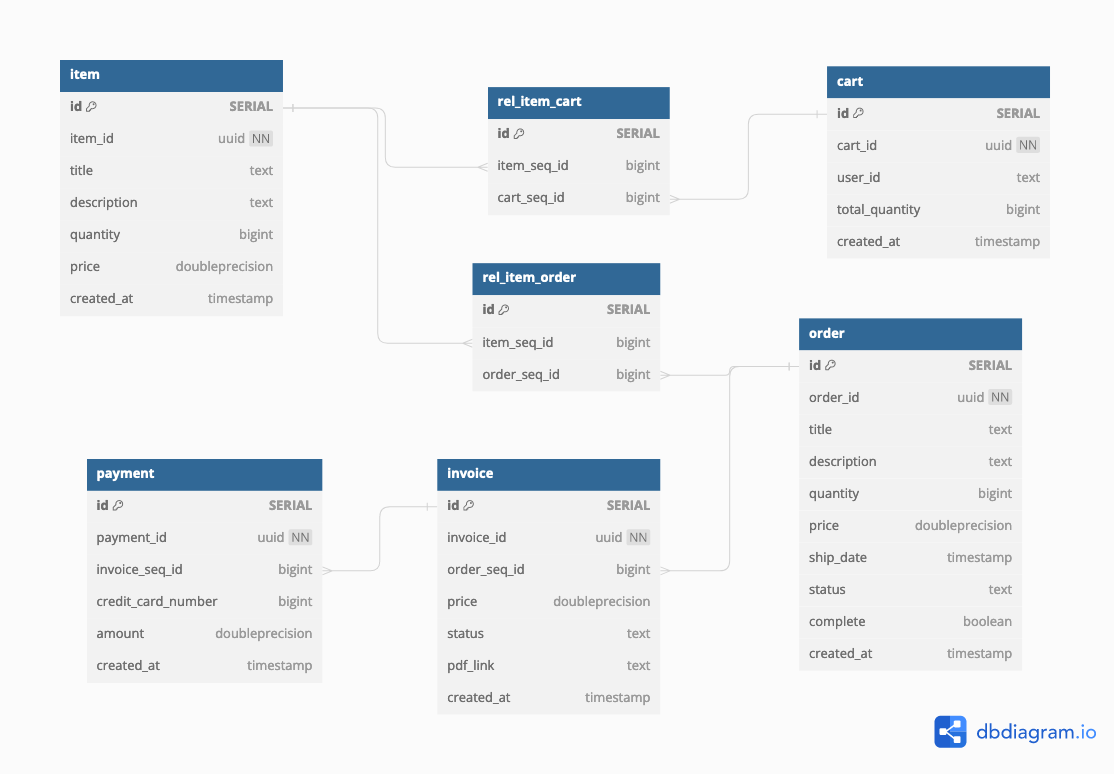
\includegraphics[width=\textwidth]{images/monolith_db_schema.png}
    \caption{Database schema displaying tables and relations of Monolithic example. \label{img:monolith_db_schema}}
\end{figure}



\section{Modulith example}
This is an example of using the modular monolith approach. The original monolithic application has been split into several smaller monoliths called \textit{modules}. The size of each module depends on the specificity of the project. In this case, it is almost equivalent to one module per database entity, except for the shopping cart and items, which have been merged into a single module to demonstrate the possibility of having modules with a larger volume. Package schema and dependencies are shown in diagram~\ref{img:modulith_package}.

Each module has the same internal structure as the original Monolith plus exposes its API with an interface (Diagram~\ref{img:modulith_module_package}). Modules encapsulate their own data storage, and there should be no cross-module table constraints in the database, although this is possible, it doesn't make sense from a logical separation perspective. It should be possible for each module to use a different database and even a different database technology. In the case of the largest module, which contains the shopping cart and items, foreign key constraints are preserved because it resides within a single module.

Modules can use API of other modules, although this should be limited as much as possible to keep coupling low. The dependency on other modules is defined through the use of interfaces, and the actual implementation can either be automatically injected using the IoC approach, or as in this case, just define a top level module that takes care of initialising individual modules and spinning up a single HTTP server.

Scaling Modulith once we have identified the bottleneck packages is very easy. Since each module is essentially a small monolith, it can be moved into service and run independently. It just needs to expose its API over the network, such as gRPC or just a simple HTTP API. This network exposure can be generated automatically if all objects in the interface are serialisable. Later client instances will be passed to all dependent modules and from the point of view of other modules nothing changes, only now the underlying communication will not be inter-process communication but network communication. The implementation could even be fully automated in a declarative way. The package can be moved to a separate service and scaled, simply by changing the configuration.

In this particular example, the implementation to expose the capabilities defined in the invoice interface was created manually by defining the following additional HTTP endpoints and thus implementing a client to satisfy the existing interface.

\begin{itemize}
    \item \textbf{Post /invoice} - Generate invoice for order specified in body.
    \item \textbf{Patch /invoice/\{invoiceId\}} - Update invoice specified by id.
\end{itemize}

The Modulith application has been extended to run in 3 modes, depending on the value of environment variables. In the first mode it runs as a single process. In the second mode it runs as a single process without invoice implementation and uses the invoice client. In the third mode it runs only the invoice implementation and this can be scaled to many instances to improve performance. Load balancing of requests to the invoice service instances is done using Nginx.

% \begin{figure}
%     \centering
%     \includesvg[width=0.7\textwidth]{images/modulith_module_package.svg}
%     \caption{Internal package structure of single module (Modulith example).\label{img:modulith_module_package}}
% \end{figure}

% \begin{figure}
%     \centering
%     \includesvg[width=0.7\textwidth]{images/modulith_package.svg}
%     \caption{Module dependency graph of Modulith example. \label{img:modulith_package}}
% \end{figure}

\subsection{Database}
Each module encapsulates its own tables, completely independent of the rest. The tables are the same as for the monolithic example on diagram~\ref{img:monolith_db_schema}, but the relations between modules have been removed. The schema consists of four partitions with relations preserved within the partition: the first partition consists of the invoice table, the second of the payment table, the third of the order table with rel\_item\_order and the last of the item, cart and rel\_item\_cart tables. Each module will have its own database pool with a maximum of 2 connections (8 in total).

% \begin{figure}
%     \centering
%     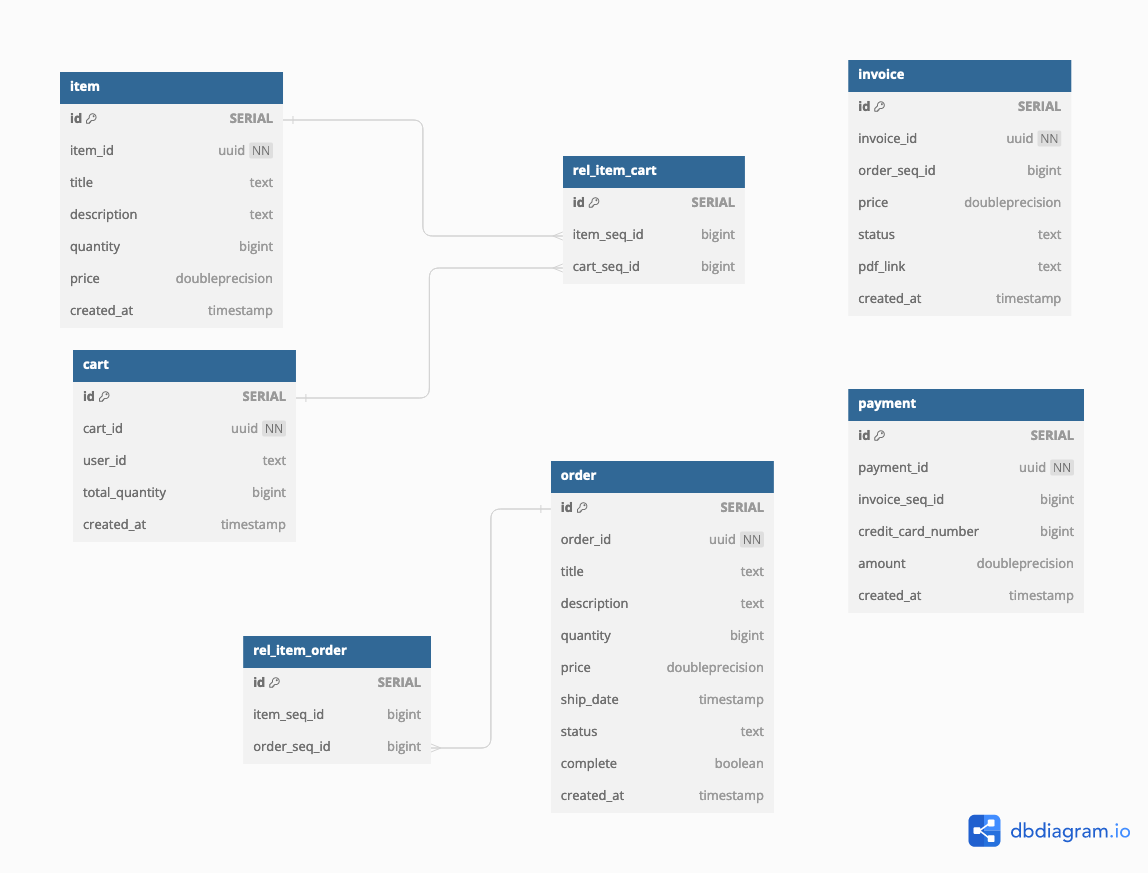
\includegraphics[width=\textwidth]{images/modulith_db_schema.png}
%     \caption{Database schema displaying tables and relations. \label{img:modulith_db_schema}}
% \end{figure}

\section{Microservices example}
In this example, the Modulith implementation has been further split into 5 microservices: Item, Shopping Cart, Invoice, Order and Payment. Modulith originally contained 4 packages, 1 of which combined the logic around Shopping Cart and Items, so it was split into two to make the scope more consistent across the microservices. The dependency graph between services is shown in Figure~\ref{img:microservices_dependency}.

Splitting Modulith into services requires exposing additional functionality over the network, as Modulith modules communicate with other modules via inter-process communication. As a result, additional endpoints (compared to the monolith) and clients had to be created to satisfy the defined interfaces.

% TODO přidat která další API musela vzniknout
\begin{itemize}
    \item \textbf{Post /invoice} - Generate invoice for order specified in body.
    \item \textbf{Patch /invoice/\{invoiceId\}} - Update invoice specified by id.
    \item \textbf{Delete /cart/\{cartId\}} - Remote cart specified by id.
    \item \textbf{Get /cart/\{cartId\}/item/id} - Retrieve item ids within cart.
    \item \textbf{Get /cart/user/\{userId\}} - Retrieve cart for user specified by user id.
\end{itemize}

Each microservice runs an HTTP server and exposes HTTP API for its internal API to be used by other modules and also public HTTP API to be used by clients. With microservices it is common to use some kind of service discovery and let services communicate directly with each other. In this example, to keep things simple, nginx was used as a load balancer, acting as an intermediary and directing requests to the right services by path matching.

The whole application is compiled into a single binary, but in production it would most likely be compiled into binaries per service. Which service is started is controlled by an environment variable.

% \begin{figure}
%     \centering
%     \includesvg[width=0.7\textwidth]{images/microservices_dependency.svg}
%     \caption{Dependency between microservices. \label{img:microservices_dependency}}
% \end{figure}

\subsection{Database}
Each microservice encapsulates its own data. The database tables are the same as for the monolithic example on diagram~\ref{img:monolith_db_schema}, but the constraints outside the microservice scope have been removed. Database partitions are the same as for Modulith, only item table has been separated into its own service after splitting one package into two separate: cart and item. Each microservice will have its own database pool with a maximum of 2 connections (10 in total).

\begin{figure}
    \centering
    \begin{subfigure}{.5\textwidth}
        \centering
        \includesvg[width=0.9\textwidth]{images/monolith_package.svg}
        \caption{Internal package structure of Monolith example. \label{img:monolith_package}}
    \end{subfigure}%
    \begin{subfigure}{.5\textwidth}
        \centering
        \includesvg[width=1\textwidth]{images/modulith_module_package.svg}
        \caption{Internal package structure of single module (Modulith example).\label{img:modulith_module_package}}
    \end{subfigure}
    % \vspace{0.5cm}
    \begin{subfigure}{\textwidth}
        \centering
        \includesvg[width=0.7\textwidth]{images/modulith_package.svg}
        \caption{Module dependency graph of Modulith example. \label{img:modulith_package}}
    \end{subfigure}%
    \hfill
    \begin{subfigure}{\textwidth}
        \centering
        \includesvg[width=0.7\textwidth]{images/microservices_dependency.svg}
        \caption{Dependency graph between microservices. \label{img:microservices_dependency}}
    \end{subfigure}
    \caption{Architecture diagrams for application examples build with architectures: Monolith, Modulith and Microservices.}
\end{figure}


\section{Benchmark methodology}
There are two types of scenarios, which will be measured to get inside into bottlenecks of applications from both CPU intensive and IO intensive perspective. Benchmarking will be done using K6 load testing tool, which will act as HTTP client sending requests defined by scenario.

Benchmarking will be done for following test scenarios with various configurations:
\begin{itemize}
    \item Performance scenario - focusing on even load of whole application testing IO and CPU intensive operations.
    \item Latency scenario - focusing primarily on IO operations and handling a lot of fast requests.
\end{itemize}

All benchmarks results will originate from running 10 parallel tests, totally 100 iterations with following configuration.
\begin{itemize}
    \item Golang 1.21.3 - programming language used for applications
    \item PostgreSQL 14 - database
    \item Docker 24.0.5 - execution environment
    \item OpenTelemetry - monitoring from within application
    \item k6 - load testing tool
    \item Hardware - Macbook Air 13" with M2, 16 GB Ram, 6 CPU cores assigned to Docker
          % TODO this configuration might change for MicroServices -> we will see
    \item Every service instance has following assigned resources unless specified otherwise: 0.5~CPU and 50~MB of Ram
\end{itemize}


\section{Benchmark results}
\label{section:benchmark_results}

\subsection{Performance scenario}
The first scenario consists of going through the whole application flow as defined on Figure~\ref{img:benchmark_flow}, which should represent evenly distributed load on the whole system. Client load list of houndred items and adds one random into his shopping cart. This repeats 10 times, after that client creates order, retrieves invoice information and pays for it. The application cosists of database queries and two harder jobs, which represents possible real world task. The first is CPU intensive task will be done during creation of order, where application generates PDF and also calculates 41st Fibonacci number to add more cpu load. The second big task, which represents waiting for 3rd party service is done during handling payment, which is implemented as 500~ms sleep.

\begin{figure}
    \centering
    \includesvg[width=0.7\textwidth]{images/benchmark_flow.svg}
    \caption{Benchmark flow diagram. \label{img:benchmark_flow}}
\end{figure}

In Table \ref{table:benchmark_baseline} are results of benchmark which will act as baseline. Both Monolith and Modulith were running in single instance with 0.5~CPU assigned and Microservices assigned 0.5~CPU per service. Even though both Monolith and Modulith are running as single process, there is already little overhead visible due to more complex internal structure and more database connection pools (separate database pool is created for every module).

\begin{table}
    \begin{tabular}{ |p{3cm}||p{3cm}|p{1.5cm}|p{1.5cm}|p{1.5cm}|p{1.5cm}| }
        \hline
        \multicolumn{5}{|c|}{Benchmark performance scenario}                           \\
        \hline
        Architecture  & Resources         & rps        & avg     & p(90)   & p(95)   \\
        \hline
        Monolith      & 0.5\,CPU, 50\,MB  & 6.8\,req/s & 1.43\,s & 1.2\,s  & 14.4\,s \\
        Modulith      & 0.5\,CPU, 50\,MB  & 7.8\,req/s & 1.25\,s & 1.59\,s & 9.18\,s \\
        Microservices & 2.5\,CPU, 250\,MB & 6.9\,req/s & 1.43\,s & 1.1\,s  & 17.9\,s \\
        \hline
    \end{tabular}
    \caption{Table containing benchmark results comparing Monolith, Modulith and Microservices. Microservices and much more CPU reserved, since it consist of 5 services (every singe one has 0.5~CPU assigned).\label{table:benchmark_baseline}}
\end{table}

The biggest bottleneck of first scenario is CPU bound task. To scale Monolith we would have to run more instances, which for big systems is very resource demanding, and target of this theses is to focus on more modern architecture styles, so it will not be discussed further. On the other hand for modulith systems it is much easier due to its modular structure. The cpu bound task is contained inside invoice package, which can be moved into separate lightweight service and scaled as much as wanted.

In second measurement invoice package was moved into separated service implementing HTTP server. HTTP client is than passed in main server to whoever module required the invoice interface. The same benchmark was run for one, two, four and eight instances of invoice service and results can be seen in Table~\ref{table:benchmark_modulith_instances} along with scaled Microservices example. There is no difference between Modulith and Modulith with single invoice service instance, but having the invoice service scaled to two instances, it has more then doubled the speed. Adding more instances scales linearly until the main bottleneck becomes IO bound task during payment. Microservices scale as well as Modulith, but having more overhead (more network inter-service communication) they are slightly slower.

\begin{table}
    \begin{tabular}{ |p{4cm}||p{1.6cm}|p{1.5cm}|p{1.5cm}|p{1.5cm}|p{1.5cm}| }
        \hline
        \multicolumn{5}{|c|}{Benchmark performance scenario}                                  \\
        \hline
        Architecture                & Resources & rps         & avg     & p(90)   & p(95)   \\
        \hline
        Modulith unified            & 0.5\,CPU  & 7.8\,req/s  & 1.25\,s & 1.59\,s & 9.1\,s  \\
        \rowcolor{Gray}
        Modulith (1x invoice)       & 1.0\,CPU  & 7.3\,req/s  & 1.35\,s & 1.0\,s  & 18.6\,s \\
        \rowcolor{Gray}
        Microservices (1x invoice)  & 2.5\,CPU  & 6.9\,req/s  & 1.43\,s & 1.1\,s  & 17.9\,s \\
        Modulith (2x invoice)       & 1.5\,CPU  & 18.8\,req/s & 510\,ms & 605\,ms & 3.1\,s  \\
        Microservices (2x invoice)  & 3.0\,CPU  & 21.4\,req/s & 441\,s  & 612\,ms & 3.9\,s  \\
        \rowcolor{Gray}
        Modulith (4x invoice)       & 2.5\,CPU  & 44.2\,req/s & 204\,ms & 521\,ms & 1.2\,s  \\
        \rowcolor{Gray}
        Microservices  (4x invoice) & 4.0\,CPU  & 58.3\,req/s & 165\,ms & 513\,ms & 1.0\,s  \\
        Modulith (8x invoice)       & 4.5\,CPU  & 71.6\,req/s & 133\,ms & 512\,ms & 0.8\,s  \\
        Microservices (8x invoice)  & 6.0\,CPU  & 66.4\,req/s & 142\,ms & 519\,ms & 0.9\,s  \\
        \hline
    \end{tabular}
    \caption{Table containing benchmark for Modulith and Microservices with module invoice moved into separate service running in multiple number of instances (indicated by number in parentheses).\label{table:benchmark_modulith_instances}}
\end{table}


\subsection{Latency scenario}
The second scenario consist just of the iterations part of previous scenario as defined on Figure~\ref{img:benchmark_flow}, but instead of repeating 10 times as in first scenario, it will repeat 100 times. Benchmark will send totally 2 000 requests (100 iterations of scenarios, 100 iterations in scenario, 2 requests per iteration), where handling of requests will consist of multiple database queries, so application will be most of the time waiting for network or database.

Benchmark will be running 100 iterations consisting of 3 http requests to retrieve list of items, add random item to shopping cart and later remove it from shopping cart. For Monolith and Modulith it is just matter of inter-process communication and database queries. In case of Microservices, there is overhead in network inter-service communication. To handle either add or remove item, there are two network requests involved: first to retrieve item data to validate if the id of item is valid and second request to load data for all item ids contained inside shopping cart.

Results of running benchmark scenario are in Table \ref{table:benchmark_scenario2}. After running initial tests, there was unexpected behavior of Monolith, which has been much slower compared to Modulith (367~req/s vs. 571~req/s). During inspecting the runtime behavior via gathered OpenTelemetry metrics, it was found out, that application used up all the available memory and was not able to process more parallel requests. Assigning it 100~MB of memory fix the issue, although it surprisingly still did not supersede the Modulith in terms of performance. Microservices had the worst performance even though they had assigned much more resources, but the benchmark is actively pressing only two microservices: cart and item, and there is the overhead of network communication between them, which has to go through the whole network stack compared to inter-process communication in other two examples. The network communication added in average 24~ms to every inter-service communication, which caused inevitable reduction in performance (four times compared to Modulith) - this metric has been measured during running benchmark using OpenTelemtry tracing.

This huge performance difference in Microservices was much more than what was initially expected around 10\,\%. After looking into tracing and resource usage statistics, the main bottleneck was evidently database, where execution time of queries ranged from hundreds microseconds up to more than 5 seconds. This has been a big surprise, since Modulith application is making exactly the same database queries, but the issue wasn't there. There came some database optimization in play where depending on order of queries database was able to optimize it and in case of Modulith application the order was just better.

\label{p:latency_issue}

\begin{table}
    \begin{tabular}{ |p{3cm}||p{3cm}|p{1.5cm}|p{1.5cm}|p{1.5cm}|p{1.5cm}| }
        \hline
        \multicolumn{5}{|c|}{Benchmark latency scenario}                                       \\
        \hline
        Architecture  & Resources         & rps        & avg    & p(90)    & p(95)   \\
        \hline
        \rowcolor{Gray}
        Monolith      & 0.5\,CPU, 50\,MB  & 367\,req/s & 6\,ms  & 51\,ms   & 67\,ms  \\
        Monolith      & 0.5\,CPU, 100\,MB & 546\,req/s & 6\,ms  & 60\,ms   & 75\,ms  \\
        \rowcolor{Gray}
        Modulith      & 0.5\,CPU, 50\,MB  & 571\,req/s & 6\,ms  & 68\,ms   & 75\,ms  \\
        Microservices & 2.5\,CPU, 250\,MB & 130\,req/s & 82\,ms & 107ms\,s & 173\,ms \\
        \hline
    \end{tabular}
    \caption{Table containing benchmark results comparing Monolith, Modulith and Microservices for second scenario.\label{table:benchmark_scenario2}}
\end{table}

All benchmarks were run on a single machine, where it does not properly demonstrate performance drawback of distributed system as Microservices are. Even though there is network communication, the latencies are pretty low compared to actually running on multiple nodes, which would add even more latency. To demonstrate this on single machine, Linux Traffic Control has been used, which is very useful Linux utility that gives ability to configure the kernel packet scheduler to modify any network property \cite{MAN_TRAFFIC_CONTROLL}. After spawning the containers the \textit{tc} command was used to set manually latency to all packets, which simulates real-world environment.

Table~\ref{table:benchmark_scenario2} contains benchmark results from running latency scenario with added extra latency to every running service. For modulith the extra latency is just on request coming from the client in both directions (inbound and outbound traffic). In case of microservices the extra latency is added for every service, so when latency is 2\,ms, the inter-service communication actually has latency 4\,ms, because two services are involved in communication. The first half of the table contains measurements of running applications with actual database, and again it shows very unexpected behavior, where Modulith with added just 8\,ms latency is performing even worse than Microservices, which was not expected at all (Modulith should be always faster due faster inter-process communication). The issue again, as in previous benchmark, has originated in database now in favor of Microservices.

To mitigate the inequality caused by database, all the database queries has been replaced by sleep for 2\,ms, which should simulated average database processing time and the results of running benchmark without database are present in seconds half of the Table~\ref{table:benchmark_scenario2_v2}. When looking on the results it is important to remind, that the benchmark is sending requests sequentially via 10 parallel clients. If it was just sending how many requests per seconds the application can handle the results would be basically the same for Modulith since the added latency would just project itself into total processing time of single request and the similar thing would happen for Microservices where it would project multiple times. But since the benchmark is running sequentially the added latency accumulates per every request thus slowing down the speed how the requests are being sent. From the results it is clear that latency negatively influences both architectures, but Microservices are more affected. Moduliths rps (requests per second) slows down by 30\,\% with added 4\,ms latency and another 40\,\% with 8\,ms latency, totalling 70\,\% slowdown, but with Microservices the situation is much worse. Added 4\,ms latency for Microservices is slowing down rps by 60\,\% (this is twice more compared to Modulith) and with 8\,ms latency another 26\,\% (notice how the another 4\,ms latency is not nearly influencing as much as the first 4\,ms, due to already big network overhead), totalling 86\,\%. The same negative effect has the latency on other metrics as well, where the average request takes for Modulith just 50\,ms and for Microservices 143\,ms, which is 2.86 times slower.



\begin{table}
    \begin{tabular}{ |p{3cm}||p{1.2cm}|p{3cm}|p{1.5cm}|p{1.5cm}|p{1.5cm}| }
        \hline
        \multicolumn{6}{|c|}{Benchmark latency scenario with database}                                 \\
        \hline
        Architecture  & Extra latency & Resources         & rps        & avg     & p(90)     \\%& p(95)   \\
        \hline
        % Weird results, resource scaling is not working
        \rowcolor{Gray}
        Modulith      & 0\,ms         & 0.5\,CPU, 100\,MB & 571\,req/s & 6\,ms   & 68\,ms    \\ %& 75\,ms  \\
        Modulith      & 2\,ms         & 0.5\,CPU, 100\,MB & 167\,req/s & 57\,ms  & 83\,ms    \\ %& 92\,ms  \\
        Modulith      & 4\,ms         & 0.5\,CPU, 100\,MB & 85\,req/s  & 57\,ms  & 164\,ms   \\ %& 183\,ms \\
        Modulith      & 8\,ms         & 0.5\,CPU, 100\,MB & 42\,req/s  & 226\,ms & 330\,ms   \\ %& 364\,ms \\
        \rowcolor{Gray}
        Microservices & 0\,ms         & 2.5\,CPU, 250\,MB & 130\,req/s & 82\,ms  & 107\,ms   \\ % & 173\,ms \\
        Microservices & 2\,ms         & 2.5\,CPU, 250\,MB & 127\,req/s & 69\,ms  & 107\,ms   \\ % & 126\,ms \\
        Microservices & 4\,ms         & 2.5\,CPU, 250\,MB & 110\,req/s & 85\,ms  & 126\,ms   \\ % & 138\,ms \\
        Microservices & 8\,ms         & 2.5\,CPU, 250\,MB & 60\,req/s  & 161\,ms & 232\,ms   \\ % & 249\,ms \\
        \hline
        \multicolumn{6}{|c|}{Benchmark latency scenario with database replaced by static 2\,ms sleep } \\
        \hline
        \rowcolor{Gray}
        Modulith      & 0\,ms         & 0.5\,CPU, 100\,MB & 668\,req/s & 14\,ms  & 17\,ms    \\ %& 21\,ms  \\
        Modulith      & 2\,ms         & 0.5\,CPU, 100\,MB & 566\,req/s & 17\,ms  & 19\,ms    \\ %& 19\,ms  \\
        Modulith      & 4\,ms         & 0.5\,CPU, 100\,MB & 457\,req/s & 22\,ms  & 23\,ms    \\ %& 24\,ms  \\
        Modulith      & 8\,ms         & 0.5\,CPU, 100\,MB & 318\,req/s & 31\,ms  & 34\,ms    \\ %& 35\,ms  \\
        Modulith      & 16\,ms        & 0.5\,CPU, 100\,MB & 200\,req/s & 50\,ms  & 54\,ms    \\ %& 54\,ms  \\
        \rowcolor{Gray}
        Microservices & 0\,ms         & 2.5\,CPU, 250\,MB & 498\,req/s & 14\,ms  & 17\,ms    \\ %& 21\,ms  \\
        Microservices & 2\,ms         & 2.5\,CPU, 250\,MB & 289\,req/s & 30\,ms  & 34\,ms    \\ %& 36\,ms  \\
        Microservices & 4\,ms         & 2.5\,CPU, 250\,MB & 202\,req/s & 46\,ms  & 50\,ms    \\ %& 53\,ms  \\
        Microservices & 8\,ms         & 2.5\,CPU, 250\,MB & 126\,req/s & 78\,ms  & 81\,ms    \\ %& 84\,ms  \\
        Microservices & 16\,ms        & 2.5\,CPU, 250\,MB & 69\,req/s  & 143\,ms & 151\,ms   \\ %& 154\,ms \\
        \hline
    \end{tabular}
    \caption{Table containing benchmark results comparing Monolith, Modulith and Microservices for second scenario.\label{table:benchmark_scenario2_v2}}
\end{table}


\section{Summary}
Three sample applications have been implemented, each using a different type of architecture. One used a monolithic architecture, the second a modular architecture and the last a microservices architecture. The different impact on the way the data has to be structured in the database and on the internal structure of the application depending on the architecture used was demonstrated. During benchmarking, the database caused unexpected application slowdown, leading to its removal and replacement with static sleep for the latency benchmark scenario to obtain more representative results.


% discuss parallel nature of Goroutines, a že většina práce je na Databázi




% TODO for microservice benchmark look into CPU usage vs modulith cpu usage
% there seems to be big spike


% \subsection{Performance}

% latency
% throughput
% scalability
% 

% \subsection{Maintainability}
% Easy debugging | logging

% \subsection{Sustainability}
% transactions?

% \subsection{Testability}

% \subsection{Complexity}




%---------------------------------------------------------------
\chapter{Methodology}
% In software engineering there is no silver bullet. Every project has its spec own specifics and requirements. Some solution can work greatly for one project and be catastrophic for others. In following text, we will look closely on architecture decision-making for projects and try to come up with straight forward methodology.

\section{Microservices are not the silver bullet}
Over the last decade Microservices architecture has gain great popularity to the extent where very little people question if this architecture is the right fit for the particular project and if there might be something better suited for the task. One reason for this might be the incredible flood of articles on the internet with primer focus on positive aspects of Microservices and how they can solve (almost) every problem, while not talking much about possible negative aspects. The important note here is that most of the articles and successful stories are in fact coming from big corporation with enormous amount of resources (e.g. Netflix, Amazon, Coca-Cola), which none of the small/medium companies can match, while also those smaller companies are facing absolutely different challenges then the inter-national corporations.

Microservices are very tightly connected to modern concept of Cloud computing, which has become multi-billion market (\$545 billion in 2022 \cite{CC_MARKET_SIZE}) with potential to bring huge savings, but also huge expenses when not used properly. And let's not pretend, those Cloud service providers are off course trying to convince us to convert into our infrastructure  and systems into new modern technologies in-order to increase their profits. This is nothing new, since everyone is just trying to make money, but we should be aware of their intentions when they are trying to convince us to use their technologies - which in case of Microservice and their complexity of operation and deployment, we will be inevitably forced to use their services, but with Monoliths we are usually capable to run everything ourselves.

In order to present some concrete data let's look into a couple of real-world examples where Microservices were not deemed as the right solution.

\begin{example}[Amazon Prime]
    An example where Microservices have proven to be too costly choice and whole application had to be migrated to Monolithic architecture in order for the system to be efficient is from Amazon. On March 22 (2023) Amazons video stream service called Prime Video, published article on their technology blog with headline `Scaling up the Prime Video audio/video monitoring service and reducing costs by 90\%'. At Prime Video, they offer thousands of live streams to their customers. To ensure that customers seamlessly receive content, Prime Video set up a tool to monitor every stream viewed by customers to identify perceptual quality issues. \cite{AMAZON_ARTICLE}

    The initial version of the service consisted of distributed components that were orchestrated by \textit{AWS Step Functions}. In there, this would allow to scale each component independently. However, the way they used components caused them to hit a hard scaling limit at around 5\,\% of the expected load. Also, the overall cost of all the building blocks was too high to use it at a large scale. The two most expensive operations in terms of cost were the orchestration workflow and data passing between distributed components. To address this issue, they moved all components into a single process to keep the data transfer within the process memory, which also simplified the orchestration logic. Since now all operations were compiled into a single process, they could rely on scalable Amazon compute (EC2) and container (ECS) instances for the deployment. \cite{AMAZON_ARTICLE}

    Conceptually, the high-level architecture remained the same. They still have exactly the same components as in the initial design (media conversion, detectors, orchestration). This allowed them to reuse a lot of code and quickly migrate. Originally, they could scale several detectors horizontally, as each of them ran as a separate microservice. However, in new approach the number of detectors only scale vertically because all run within the same instance, and it would quickly exceed the capacity of a single instance. This limitation was overcome by running multiple instances and by implementing lightweight orchestration layer to distribute customer requests. Overall the migration from distributed Microservice architecture to Monolith let them save cost of infrastructure over 90\,\% and increased scaling capabilities. \cite{AMAZON_ARTICLE}
\end{example}

\begin{example}[Shopify]
    An example of company who still run successfully Monolithic system with thousands of developers is Shopify. It is a complete commerce platform, that enables businesses to build an online store, market to customers and accept payments. The article\cite{SHOPIFY_MONOLITH_ARTICLE} with the most insights of their architecture comes from Sep 16 2020, and they are writing regularly more insight stories about their Monolith on their \textit{Shopify Engineering}\cite{SHOPIFY_ENGINEERING} website.

    They have a massive Monolith written in Ruby on Rails framework, just its core is having over 2.8 million lines of Ruby code. This is one of the oldest, largest Rails codebases on the planet, under continuous development since at least 2006. Rails doesn't provide patterns or tooling for managing the inherent complexity and adding features in a structured, well-bounded way. That's why in 2017, Shopify founded a team to investigate how to make their Rails monoliths more modular. The goal was to help scale towards ever-increasing system capabilities and complexity by creating smaller, independent units of code they called components. The added constraints on how they write code triggered deep software design discussions throughout the organization. This resulted in mindset shift across developers towards stronger focus on modular design. Clearly defined ownership for areas of the codebase was one of the key factor for successful transition. \cite{SHOPIFY_MONOLITH_ARTICLE}

    They started out by focusing on building a clean public interface around each component to hide the internals. The expectation was that changing internals of a component wouldn't break other components, and it would be easier to understand the behavior of a component in isolation. They had to balance the encapsulation with dependency graph to avoid circular dependencies, which are very risky since change to any component within chain can break all other components. Different techniques like inversion of control and publish/subscribe mechanism were introduced to helped minimize relations and decrease coupling. At the end they ended up with 37 components in the main monolith, and they are very deliberate about splitting functionality out into separate services due to overall complexity of distributed system of services. \cite{SHOPIFY_MONOLITH_ARTICLE}
\end{example}

\begin{note*}
    Netflix is one of the most mentioned company for its Microservices architecture. What is not that well know, is that the actual migration from Monolithic system, when they started to having trouble with performance and scaling was in 2009. By that time they had Monolith for 10 years and in that time already over 11~millions \cite{NETFLIX_2009_EARNINGS} of paying subscribers. No one knows what would happen if they started the original architecture with something else, maybe it would work, but definitely the Monolith worked well until it just didn't suit their need anymore.
\end{note*}

\section{Decision making}
Every software project composes of at least 6 stages: planning, designing, development, test, deployment, and maintenance. We will be primarily discussing the first two: planning and designing, because that is where the high level decision around architecture is made. Ideally, a software architect creates the concepts and designs for software and helps turn those concepts into plans, just like an architect who designs buildings. In smaller projects, the role of software architect will usually fall on the most experience developer. While building architects are not typically concerned with how their ideas are implemented, a software architect is engaged throughout all stages of the development process, not just around architecture, but all high-level decisions regarding tools, coding standards or platforms to be used.

The architecture of the system is probably the most important decision to be made, since it influences all following stages of development and usually presents quite the challenge to change afterwards. Interestingly, choosing the architecture is not just about meeting all the projects requirements, but it also must fit into the style of the organization. There is an IT theory created by computer scientist/programmer Melvin Conway in 1967, which states: ``Organizations, who design systems, are constrained to produce designs which are copies of the communication structures of these organizations.''\cite{paper:conway:1968}. And this theory makes a lot of sense. When we are making any hard decision, we are always more incline to something we know well, rather than something what could be better, but we have zero experience with. Also, not all the designs might be compatible with our organization structure. For example Monolith with 4 month release cycle won't for early stage startup, where they are adding new feature every week into their product and working in short iteration cycles. The same applies other way around. Having Microservice architecture, fast iteration cycles and ability to deploy whenever some feature is ready is great, but when applied in a corporation with complex hierarchical structure, where getting approved simple changes takes weeks does not even remotely utilize the benefits the architecture has to offer.

The importance of choosing correct architecture for many software projects is being underestimated and influenced by new shining trends and fancy words in IT industry instead of being primarily driven by requirements, and it can lead to unstable, inefficient and overpriced projects.

\subsection{Choosing right criteria}
To be sure that the chosen software architecture will meet the needs of the software that will be developed, it is very important that the architect fully grasps and understands the business needs that will be served. All of those should be as equality understood as the technical and functional expectations of the application. The general aspects to consider:
\begin{itemize}
    \item Security and performance requirements
    \item Client and vendor expectations
    \item The type of hosting
    \item Technologies
\end{itemize}

To build good requirements, as much questions as possible have to be answered. It is imperative that all requirements are defined in most specific and concrete way. Having vague and unattainable requirements is nearly as good as have none. It's not enough to say performance, portability or scalability. No project can have absolutely perfect performance. It must be properly specified and also limited in order to meet other requirements as well\cite{REQUIREMENTS_LIMITED}.
% TODO přidat diagram x dimenzí a že nelze každou mít na 100, ale je třeba kompromisů - fancy diagram nevím jak se jim žíká

Requirements are generally divided into two categories:
\begin{itemize}
    \item \textbf{Functional requirements} describe what a system has to do. If the system does not meet functional requirement it will fail. This is because it is not being able to do something it must do to operate properly. Another way to view functional requirements is in terms of inputs and outpus.They specify what the system must to do in response to different inputs and what it must output.
    \item \textbf{Non-functional requirements} describe how the system works. They focus on how the system delivers the specified functionality. At a first glance, they may seem as less important than functional requirements, but both are significant. Non-functional requirements do not have influence on functionality of the system, but they have impact on how well it will be performed.
\end{itemize}

Another thing which might influence the decision is team experience. If we have team of developers with great deal of experience in creating Monoliths and zero experience with distributed system, choosing Microservice architecture as a starting point can prove to be decision, which we might regret. Microservices require completely different mindset than to which the team were used to while building Monoliths. And we might easily end up with something which should be avoided at all cost: \textit{distributed Monolith}.

\section{Modulith lifecycle}
Architecture ability to adapt in the long run to different requirements is an important quality. Modulith stands right between Monolith and Microservices, which gives it ability to easily convert forth and back between different architecture styles. The following text describes few examples on how the Modulith can utilize.

% Monolith -> Modulith, mnohem snažší a iterativní oproti Monolith -> Microservice
\subsection{Monolith to Modulith}
\label{subsection:monolith_to_modulith}
Lot of the software companies, who has been around for few years and did not jump fully into Microservice hype right away do have some legacy Monolithic systems, whose maintenance is costly, but they cannot be converted into Microservices, since it would require rewriting the whole system from the ground up and no one from business wants to make this kind of big investment which would basically not bring any new feature.

Instead of this radical approach of rewriting the whole system, which will basically cost the company twice the money, since rewriting system means creating new project with all steps of development: analyses, design, etc. and long period of bug fixing. I would rather suggest iterative approach of converting existing Monolith into Modulith, by concentrating on solving specific issue at hand, rather than trying to solve everything at once by rewriting the application. The method is displayed on Figure~\ref{fig:monolith_to_modulith_steps} and consists of following steps:

\begin{enumerate}
    \item \textbf{Modularization} step impose restructuring code and modularizing the whole application, yet without worrying about issues associated with Distributed system (network reliability, latency, complexity). Proper focus can be invested into determining modules, their responsibilities and boundaries. Depending on the project the scope of modules can vary from complex modules to single responsibility per module.
    \item \textbf{Scale unit} step is about getting the application ready for scaling by running multiple instances. Monolithic systems are Usually stateful or require some kind of synchronization for part of its functionality. In this step all of those either potential or actual blockers of running multiple instances needs to be solved or replaced by solutions which can scale. Now the application can achieve high availability and increase performance by scaling the whole instance. Now the architecture reached the definition of Modulith.
    \item \textbf{Scale modules} step takes ability to scale even further by allowing to scale individual modules or group of modules instead of the whole application as a unit. This should be implemented with scare, since it might not even be needed as long as scalability reached by previous step is sufficient, and also it introduces significant negative effects:
          \begin{itemize}
              \item Becomes distributed system - network instability, higher latency, complexity, complicated debugging and logging.
              \item More complicated deployment - some sort of versioning is required to ensure compatibility between individual modules.
              \item More code or tooling - instead of just having interfaces and its implementation to separate modules, now it has to be also implemented to support network calls, so some client/server code has to be implemented or ideally generate by additional tools.
          \end{itemize}
          By completing the Scale modules step, the architecture reaches state defined as \textit{Hybrid Modulith} in this theses.
\end{enumerate}

\begin{figure}
    \centering
    \begin{subfigure}{.5\textwidth}
        \centering
        \includesvg[width=0.5\textwidth]{images/monolith_to_modulith_0.svg}
        \caption{Original Monolith}
    \end{subfigure}%
    \begin{subfigure}{.5\textwidth}
        \centering
        \includesvg[width=0.7\textwidth]{images/monolith_to_modulith_1.svg}
        \caption{Modularization step}
    \end{subfigure}
    % \vspace{0.5cm}
    \begin{subfigure}{\textwidth}
        \centering
        \includesvg[width=0.4\textwidth]{images/monolith_to_modulith_2.svg}
        \caption{Scale unit step (reached Modulith)}
    \end{subfigure}%
    \hfill
    \begin{subfigure}{\textwidth}
        \centering
        \includesvg[width=0.7\textwidth]{images/monolith_to_modulith_3.svg}
        \caption{Scale modules step (reached Hybrid Modulith)}
    \end{subfigure}
    \caption{Conversion steps from Monolith to Hybrid Modulith}
    \label{fig:monolith_to_modulith_steps}
\end{figure}

% Modulith scaling, přidávání instancí a rozdělení Modulithu (lze dělit na různě velké celky)

% Modulith -> Microservice, multiple teams, want to add network boundaries and more granular responsibility distribution
\subsection{Modulith to Microservice}
Over the time the Modulith architecture might stop suiting the needs of the project. Examples reasons: more gine-grained granularity of the application is required, teams need to have more independents, missing technology-agnosticism or more distributed solution is wanted to achieve higher availability or scalability.

After properly weighting all pros and cons, decision can be made to migrate Modulith to Microservice architecture. The transformation should come ideally as natural steps over time with changing requirements and system needs. Modulith is composed of individually scalable modules with defined boundaries. Moving to Microservice architecture is about refining those modules and transforming into microservices via defining fine-grained boundaries. In cases where modules were defined with small scopes, the transformation can be simply 1 module to 1 microservices, but usually modules will be split into multiple microservices, since they have larger scope compared to Microservices which are usually driven by single business responsibility principle. The example transformation step is shown at figure~\ref{fig:modulith_to_microservices_steps}.

\begin{figure}
    \centering
    \includesvg[width=\textwidth]{images/modulith_to_microservices_steps.svg}
    \caption{Conversion step from Modulith to Microservices.\label{fig:modulith_to_microservices_steps}}
\end{figure}


% Microservice -> Modulith, sloučení služeb sníží overhead, zjednodušší vývoj, vhodně pro menší týmy
\subsection{Microservice to Modulith}
% pozn. různé technologie/jazyky
Microservice architecture can become too complex to manage or just too expensive to operate. The solution might be in converting Microservices into Modulith, which will simplify deployment resulting in cheaper infrastructure and boost up developer productivity by removing complexity of distributed system.

The migration is done simply by converting microservices into modules as shown at Figure~\ref{fig:microservices_to_modulith_steps}, since they are already fully encapsulated and have defined API. The network communication can be completely replaced by inter-process communication or if for some modules scalability is required for performance, it can be converted into \textit{Hybrid Modulith} as specified in \textit{Scale modules} step of section~\ref{subsection:monolith_to_modulith}. Later on some modules might merge together to take on bigger responsibility, but this depends on how the module boundaries are set within project.

\begin{figure}
    \centering
    \includesvg[width=\textwidth]{images/microservices_to_modulith_steps.svg}
    \caption{Conversion step from Microservices to Modulith.\label{fig:microservices_to_modulith_steps}}
\end{figure}


\section{Building a new application}
When building an application from ground up, I believe the Modulith is currently the best/safest choice. Because why everyone is choosing Microservices from the start? Because of performance? On start of project we have some presumptions about performance requirements, but they are still just `presumptions' and actual performance issue in most cases are inflicted by limitations of the actual implementation. Also, the performance requirements might dramatically change once the business moves in some other direction than expected at the start and this is something which happens a lot in startups.

So it might be the independence of microservice? The Modulith offers the same quality with modules. Just the Microservice are more dramatically enforcing smaller scope, which can be leveraged for modules in the same manner. How about testability? Again, modules can be tested in same independent manner as Microservice plus even further using techniques known from Monoliths like end-to-end testing without all the shenanigans connected with Microservices and orchestrations. Maintainability? Modulith has much simpler deployment strategy, less complex environment and are cheaper to host. Sustainability? The amount of work required to just merge two Microservices into single one is quite high, due to inability to effectively even find all of its defendants and update them all accordingly. On other hand since Modulith is just single codebase, the relations are there and visible just by using standard and proven tools e.g. IDE with `find usage' feature. Also, any deep refactoring can be done in Modulith in much easier manner than in Microservice. The biggest negative aspects for small/medium projects lies in ability of developers to properly defined scope and boundary of modules and more importantly preserving it over the time, since the individual microservices have network boundary which is hard to cross, but with Modulith it is much easier, since it is one repository with inter-process communication, but this can be largely avoided by setting up automated tools, which will enforce the boundaries on code level directly by monitoring cross-module dependencies. The recommended lifecycle of the project can look like this:

% vývojáři musí správně nastavit scope a boundaries, složitější uhlídat, musí se správně nastavit ?procesy?

\begin{enumerate}
    \item Properly defined scope and boundaries of individual modules
    \item Build the Modulith and scale as unit until it is efficient.
    \item Identify modules having performance issues and move them into independent service (another Modulith).
    \item Scale the independent Moduliths as required.
    \item In case of need for additional granularity migrate to Microservices architecture.
\end{enumerate}


% TODO: At the start of planning phase, all criteria which will drive the decision should be specified, so they can be later used to transparently compare different solutions and choose the best of them. 

% Overlooked importance of choosing right architecture, leads to instability, insifficency and hight costs
% to undestood, architect must fully grasps business needs 
% - describe architect and his role in software design 
% - quote M. Conway, a computer scientist, once said: “Organizations which design systems ... are constrained to produce designs which are copies of the communication structures of these organizations.” This is a clear guideline for architects to take into account the company structure when designing new solutions. 

% záleží i na týmu - každý má jiné zkušenosti a znalosti -> bude trvat než se adaptují
% Choosing criteria - list
% functional and non-functional requirements

% be awera of over-engineering
% Prototype, iterations - fail fast

% Sources https://www.bocasay.com/web-application-software-architecture/
% https://dl.acm.org/doi/epdf/10.1145/1978802.1978812 (první article na decision making)
% - Hence architects should choose a decision-making technique based on the difficulties that they wish to avoid. (začátek)
% - Software architecture determines not only how the system should be constructed, but also guides its evolution
% https://www.lucidchart.com/blog/how-to-design-software-architecture
% - It’s not enough to say you want performance, portability, or scalability, though. Non-functional requirements must also be quantified. No project can have absolutely perfect performance: “performance” must be specified and limited in order to meet other requirements. 


% Přidat několik praktických příkladů s úvodem, různými architekturami a možnými následky % include `text.tex' from `text/' subdirectory

\appendix\appendixinit % do not remove these two commands

\chapter{Nějaká příloha}


Sem přijde to, co nepatří do hlavní části.
 % include `appendix.tex' from `text/' subdirectory

\backmatter % do not remove this command

\printbibliography % print out the BibLaTeX-generated bibliography list

\chapter{Obsah přiloženého média}


	\dirtree{%
		.1 readme.txt\DTcomment{stručný popis obsahu média}.
		.1 exe\DTcomment{adresář se spustitelnou formou implementace}.
		.1 src.
		.2 impl\DTcomment{zdrojové kódy implementace}.
		.2 thesis\DTcomment{zdrojová forma práce ve formátu \LaTeX{}}.
		.1 text\DTcomment{text práce}.
		.2 thesis.pdf\DTcomment{text práce ve formátu PDF}.
	}
 % include `medium.tex' from `text/' subdirectory

\end{document}
